%-------------------------------------------------
%-------------------------------------------------
% Preamble
%-------------------------------------------------
%-------------------------------------------------

\documentclass[12pt]{article}
\bibliographystyle{unsrtnat1}
\usepackage[numbers]{natbib}
\usepackage[english]{babel}
\usepackage [autostyle, english = american]{csquotes}
\MakeOuterQuote{"}
\usepackage{times}
\usepackage{verbatim}
\usepackage{placeins}
\usepackage{cancel}
\usepackage[justification=centering]{caption}
\usepackage{listings}
\usepackage{color}

\definecolor{gray}{rgb}{0.5,0.5,0.5}
\definecolor{mauve}{rgb}{0.58,0,0.82}

\lstset{frame=tb,
  language=Python,
  aboveskip=3mm,
  belowskip=3mm,
  showstringspaces=false,
  columns=flexible,
  basicstyle={\small\ttfamily},
  numbers=none,
  numberstyle=\tiny\color{gray},
  keywordstyle=\color{blue},
  commentstyle=\color{red},
  stringstyle=\color{mauve},
  breaklines=true,
  breakatwhitespace=true
  tabsize=3
}

\usepackage{graphicx}
\graphicspath{{C:/Users/Kyle Shank/Desktop/SCHOOL/COA/SENIOR PROJECT/Write Up Files/pictures/}}
\usepackage[pdfauthor={Author's name},%
pdftitle={Document Title},%
pagebackref=true,%
pdftex]{hyperref}
\usepackage{amsmath,amsthm,amssymb}
\usepackage[doublespacing]{setspace}

%-------------------------------------------------
%-------------------------------------------------
% Document Header
%-------------------------------------------------
%-------------------------------------------------

\begin{document}
\title{Evaluating methods for detecting critical transitions in agent-based models}
\author{Kyle Scot Shank\\
  College of the Atlantic\\
  Senior Project, Spring 2014\\
  \texttt{kshank@coa.edu}}
\date{\today}
\maketitle
\thispagestyle{empty}
\newpage

%-------------------------------------------------
%-------------------------------------------------
% Abstract
%-------------------------------------------------
%-------------------------------------------------
\begin{abstract}\noindent
There are many examples of unexpected and rapid change in terrestrial and marine ecosystems: the dramatic shift from vegetated savanna to open desert in the Sahara during the early Holocene, the unexplained disappearance of Atlantic cod from the coastal waters off Newfoundland in the 1990s, or the ongoing problem of colony collapse disorder effecting pollinator communities worldwide. Such catastrophic collapses, also known as critical transitions, may sometimes be presaged by early warning signals that could be used to predict and potentially prevent such events. Though several generic early warning signals have been proposed in the literature, there are open questions regarding the universality of such signals across a variety of ecological models and model specifications. Moreover, there is little research exploring the discovery of critical transitions and their early warning signals in agent-based ecological models. Here, I present evidence that the presence of early warning signals may be dependent upon the choice of modeling paradigm. I use a relatively simple ecological model with a critical transition known to be "silent" (i.e.,  does not show early warning signals) to construct an agent-based model of the same dynamics and analyze the presence of early warning signals in both modeling environments. I propose that the theory regarding critical transitions be expanded to include analyses of particular issues facing the discovery early warning signals and critical phenomena in agent-based models. Additionally, a comparison of early warning signals detection between differential equation-based and agent-based modeling paradigms may have many applications for ecological management.
\end{abstract}
\newpage
%-------------------------------------------------
%-------------------------------------------------
% Body
%-------------------------------------------------
%-------------------------------------------------
\tableofcontents
\newpage
%-------------------------------------------------
%-------------------------------------------------
%-------------------------------------------------
%-------------------------------------------------
% SECTION ONE
%-------------------------------------------------
%-------------------------------------------------
%-------------------------------------------------
%-------------------------------------------------
%-------------------------------------------------

% Introduction
%-------------------------------------------------
\section{Introduction}
It is well-known that models of many ecological systems exhibit large-scale, discontinuous change which may represent shifts between alternative stable states \cite{Holling1973}\cite{May1977}. The case of eutrophication in shallow lakes is a powerful example: a lake may rapidly shift from a vegetation-dominated clear state to a more turbid phytoplankton-dominated state due to nutrient loading, removal or loss of certain species of submerged vegetation (also known as \emph{macrophytes}), or a change in population dynamics due to the  introduction of additional predators into the environment \cite{Scheffer2009c}\cite{Wang2012}. Such sudden shifts are not strictly limited to ecological settings. There are examples of rapid succession events in climate models, such as in the conjectured collapse of the thermo-haline circulation during the Younger Dryas period \cite{Dakos2008} or many of theories surrounding "Snowball Earth" \cite{Scheffer2009c} (both of which entail a rapid shift, in geological terms, from a relatively warm, wet period to one that was significantly colder and drier). Similar phenomena are also found in human systems, exemplified quite well by the recent collapse of the global financial system
	\footnote{The argument here is that the two states are one of high liquidity and "easy" credit and one of low liquidity and unavailable credit. However, there is ample evidence 
	that financial markets may be significantly more complex \cite{Hsieh1991}\cite{Johansen2000}.} \cite{Haldane2011}
but also extending into theories regarding the breakdown of coupled social-ecological systems, such as the colony collapse disorder currently plaguing economically and ecologically critical pollinator species \cite{JelleLever2014}.\\

Such sudden events are referred to by variety of names in the scientific literature and popular science: catastrophic bifurcations, regime changes, tipping points, and critical transitions. Taking into consideration not only the examples mentioned above, but also the generally increasing rate of species extinction events, rapid environmental changes, and the growing global interconnectedness (and subsequent turbulence) of the economic and financial spheres, a keen interest in the study of such critical transitions is of little surprise \cite{Scheffer2009a,Dakos2013a}. Within this expanding field, it has been theorized (mainly by ecologists) that there may be a level of universality in the ability to discover "early warning signals" for such events \cite{Scheffer2001,Drake2010,Dakos2012,Wang2012,Carpenter2011,Chisholm2009,Scheffer2012}. Such early warning signals would be of paramount interest to the management of a variety of ecological systems. As avoiding catastrophic collapse requires the ability to predict critical transitions in advance, the importance of being able to clearly recognize signs of an impending shift cannot be overstated. Additionally, even if such events cannot be avoided, adaptation and mitigation might require an ability to predict a shift prior to its occurrence if the time scale of implementation is sufficiently long relative to the rate at which damages occur \cite{Boettiger2013}. \\

These theoretical findings  have not come without their criticisms \cite{Boerlijst2013}\cite{Boettiger2013a}\cite{Hastings2010}, many of which are directed toward the mathematical foundations of both the models being presented and the means by which researchers have claimed to have discovered their various early warning signals. Such criticisms must be addressed, and will be, as they become relevant to the problem below. However, before further discussion of early indicators and their criticisms, I will give a more concrete definition of both critical transitions and early warning signals.

%-------------------------------------------------
% Critical Transitions
%-------------------------------------------------
\subsection{Critical Transitions}

The use of the term critical transition (which will be used exclusively hereafter) to describe abrupt system transitions is closely linked to an expanding group of theoretical ecologists, including Scheffer, Carpenter, Levin, and Dakos. The phenomenon itself, however, has been known to fields of thermodynamics and dynamical systems for some time \cite{Yang1952}\cite{Wissel1984}\cite{Strogatz2000}. To offer an intuitive definition, a critical transition can be thought of as the threshold between two states in a given system. Take, for example, the overall attitude of a gathering crowd at a protest. In one state, the crowd is peacefully demonstrating. However, if enough external forcing is applied (such as, perhaps, by water cannon, or some other police behavior) the crowd may shift into a far more riotous state of being. Examples of such sudden shifts abound in sociological and ecological settings: the switch of sentiments from positive to negative as expressed in blog posts \cite{Slater2012}, the availability (or lack thereof) of keystone predators in fisheries models \cite{Beninca2008}, or the transition of Amazonian rainforest from a moist state to an arid one under climatic pressure \cite{Boulton2013}. The critical transition, then,  is simply the abrupt change that occurs between such states.

To be a bit more precise, a critical transition is the rapid change of a time-dependent system between two basins of attraction. Such behaviors are illustrated schematically in Figure 1.

\begin{figure}[!htb]
\centerline{
\begin{centering}
\minipage{\textwidth}
  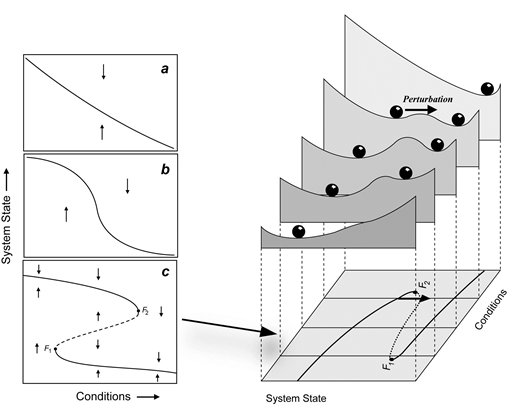
\includegraphics{tippingpoints.jpg}
  \caption{Graphical representation of how critical transitions may happen at tipping points (see text). Image is from the Synergy Program for Analyzing
Resilience and Critical Transition (SparcS, \texttt{www.sparcs-center.org}).} 
\endminipage
\end{centering}
}
\end{figure}
\FloatBarrier

In Figure 1, the "system" may be thought of as the landscape that the ball (our variable of interest) is traversing. The ball may be rolled within its current basin, or (if rolled hard enough) cross over a threshold from one basin to another. What's important to note is that on the right hand side of the figure, we see that the shape of the basin \emph{changes} as the conditions of the system are changed: depending upon how the interactions of the system state (the $y$-axis) and the system conditions (the $x$-axis) play out, the ball may shift from one basin to another will relative ease, or (more importantly) the separate basin might completely disappear and the ball might transition to a new, permanent state. When these transitions are particularly sudden, we call that shift a critical transition \footnote{Box c also exhibits the phenomenon of \emph{hysteresis}. In technical terms, hysteresis is the dependence of the output of a system not only on its current input, but also past inputs. In terms more fitting to our critical transition framework, it simply means that it may take more "force" to push a system back into a previously stable state after it has crossed the critical transition threshold.}. \\

For our purposes, we will also hold two basic assumptions about the kinds of systems that we are interested in. First, the underlying process is deterministic,\footnote{A system is \emph{deterministic} if there is no randomness involved in the development of that system over time. Using our example of the crowd at a protest once again: the system is deterministic because we hold the assumption that the crowd will not spontaneously begin to riot (i.e., we are assuming the non-existence of rabble-rousers in the population). This does not necessarily imply, however, that the outcome of a deterministic is \emph{predictable}. Chaotic systems, such as the weather, are also deterministic, but their sensitive dependence on initial conditions means that even the smallest bit of measurement error can cause radically different system outcomes \cite{Strogatz2000}.} but potentially subject to some degree of random fluctuations (known as \emph{stochastic forcing} or \emph{environmental noise}). Second, the transition occurs rapidly compared to the temporal scale of the current state dynamics. For example: the time-scale of our protest (days and weeks) may be an a order of magnitude longer than the time-scale of the disturbance (hours or minutes, depending on the severity of the riot-control measures) \cite{Kuehn2013}. \\

Though such phenomena may be easily observable after the fact, critical transitions are notably difficult to classify and predict. The system may appear to be under normal conditions and suddenly shift without warning or suffer a "silent catastrophe" \cite{Boerlijst2013}, or the complexity of the system being modeled may be so great as to prohibit accurate identification of dynamic change and fluctuations \cite{Green2005}. Despite these difficulties, research \cite{Scheffer2012}\cite{Seekell2013} has shown that many different ecological systems display similar behavior when in the vicinity of a critical transition point. These behaviors, hereafter referred to as early warning signals (EWS), are based upon several well-known mathematical techniques borrowed from dynamical systems theory, bifurcation theory, mathematical statistics, and time-series analysis. Though an increasing number of generic early warning signals have been proposed in the literature, we will focus on only a few: increasing autocorrelation, increasing variance and coefficient of variation, increasing skewness and kurtosis, and spectral reddening.

%-------------------------------------------------
% Early Warning Signals and Critical Slowing Down
%-------------------------------------------------
\subsection{Early Warning Signals}

The most well-studied EWS for a critical transition is critical slowing down (CSD), which in ecological terms may be thought of as a decline in the overall "resilience" of an ecological system as it gets close to a point of transition \cite{Carpenter2012}. We define ecological resilience here as the ability of a system to absorb external shocks and perturbations and persist at a particular stable equilibrium point. As this type of resilience cannot be directly measured (in a quantitative sense), we instead look for indirect indicators of change. The strongest of these indicators is an increase of repeated system behavior over short intervals (also known as increasing \emph{autocorrelation} \footnote{More explicitly defined, autocorrelation is the correlation between successive values of the same time-series, or the cross-correlation of a signal with itself \cite{Chatfield2000}.}) and increasing variance in the time-series of the system as it approaches a critical transition \cite{Holling1973}. In less technical terms, we thus measure resilience by how quickly a shock to a sytem dissipates. If the shock persists in the system for some time (manifested as subsequent observations that become more and more similar), we may then say that the system's "memory" is becoming "long" and we are observing CSD. \\

As disturbances occur, the rate at which the system recovers from small shocks becomes increasingly slow and drawn out. This "slowing down" of the system as it nears a critical transition is reflected as an increase in the short-term (low lag) autocorrelation of the time-series. \footnote{
	Autocorrelation is calculated as follows. Let $X$ be some repeatable process, and $i$ be some point in time after the start of that process. Then $X_i$ is the value  produced by a given run of the process at time $i$. Suppose that the process is further known to have defined values for mean $\mu$ and variance $\sigma^2$ for all times i. Thus, the autocorrelation ($R$) between time $t_1$ and $t_2$ is $R(t_1,t_2) = \dfrac{\text{E} [(X_{t_1} - \mu_{t_1})(X_{t_2} - \mu_{t_2})]}{\sigma_{t_1}\sigma_{t_2}}\,$ where E is the expected value operator.}
Specifically, an increase in \emph{autocorrelation at-lag-1} (or "ar(1)") may indicate that the state of the system has become increasingly cross-correlated with itself between consecutive observations. Less formally, this may indicate that subsequent observations in the time-series are increasingly related to previous observations, or that the system's "memory" is increasing. Thus the current length of the system's "memory" may reveal information about the system's ability to respond to further environmental forcing \cite{Dakos2012}. \\

Slowing recovery rates near a critical point may also make the system drift widely around the stable state space. As the impacts of small shocks do not decay, their accumulated effect may increase the \emph{variance} of the state variable \cite{Scheffer2009a} as it finds itself spending more and more time at what would be otherwise "extreme" values under normal conditions. Thus, increasing variance, measured either as standard deviation (how much a value varies from the average) or the coefficient of variation (the extent of variability in relation to the mean of the population, where $\left.c_v = \dfrac{\sigma}{\mu}\right)$, may serve as a useful indicator of an approaching critical transition.\footnote{There is some evidence that critical slowing down could have the opposite effect on variance \cite{Berglund2002}. As this evidence is inconclusive and we are utilizing a variety of EWS, we will assume that variance will increase as our model approaches a critical transition}. \\

\emph{Skewness} and \emph{kurtosis}, the third and fourth moments of a statistical distribution, may also be useful indicators. As explained above and  in \cite{Dakos2012}, disturbances may increase the system variance and bring it nearer to the transition boundary. As this occurs with a higher degree of frequency and the dynamics of the system as it nears that boundary slow down, we may observe a change in the skewness, or asymmetrical distribution of values, in the time-series. That is, if we looked at a histogram of values for the time-series, we would see an asymmetrical shift towards "extreme" values. \footnote{Note that we are seeking for \emph{change} in skewness, not necessarily an increase or decrease. Skewness may increase or decrease depending on whether the transition is moving towards an alternative stable state that is larger or smaller than the current state \cite{Scheffer2009a}.}\\

Measurement of kurtosis, or the "peakedness" of the distribution curve, may also prove to be a useful EWS. Since random shocks and environmental noise may make it more likely that the state of a system will find extreme values, the distribution of the time-series may exhibit positive kurtosis, also known as being \emph{leptokurtic}, signaling that the tails of the distribution have become "fatter" due to the increased presence of rare values in the time-series \cite{DeCarlo1997}\cite{Biggs2009}. These statistical moments may at first glance seem dauntingly complex and obtuse, but their value for detecting critical transitions is easy to explain. From a statistical point of view, whenever large deviations from the "normal" state of the system become more and more frequent, it becomes increasingly likely that the system in question is about to deviate from what was previously thought of as "normal" behavior. Skewness and kurtosis are well-understood (and relatively easy to calculate) indicators of such change.\\

Lastly, power spectrum analysis may be utilized to search for \emph{spectral reddening}, another in our suite of EWS. A power spectrum analysis describes how the overall variance of the system is distributed by decomposing the variation into different frequencies \cite{Chatfield2000}. A system that is closer to a critical transition tends to show spectral reddening, or a shift from dominance by high frequency processes to low frequency processes, and an increase in the amplitude of fluctuations \cite{Biggs2009}\cite{Kleinen2003}. This can be measured in a variety of ways, but one of the most computationally straightforward is by estimating the spectral density ratio. The spectral density ratio describes how variation in the data may be accounted for by cyclical components of different frequencies as determined by Fourier analysis. Following \cite{Biggs2009}, we define the spectral density ratio as the ratio of low frequency processes (cyclical components with a wavelength$ = 0.05$) to the spectral density at a high frequency (cyclical components with a wavelength $= 0.5$).\\

Though we will be searching for the above EWS in our investigation, we do not seek to imply that other conjectured EWS are less generalizable. For a more thorough overview of early warning signals, please refer to \cite{Dakos2012} and \cite{Lade2012}. As has been shown, there is a wealth of literature investigating EWS in a variety of model specifications. Many of these models are expressed as systems of coupled ordinary differential equations (ODE) to produce time-series for analysis. Yet there are a variety of ways in which to model theoretical ideas and empirical findings, of which ODE models are but one example. Another that I will focus on will be agent-based models, which are of growing importance and prominence in ecology \cite{Grimm2005}\cite{Parunak1998}. 

%-------------------------------------------------
% Agent-based Models in Ecology
%-------------------------------------------------
\subsection{Agent-based Models in Ecology}
An agent based model (ABM) is a type of computational model which simulates the actions and interactions of individual agents in order to observe the aggregate effect of autonomous behavior on the system as a whole. By agents, we are referring to individuals (which may represent actual individuals or groups) within an environment that have behaviors based on certain rules. Such models stand in contrast to models  based on equations where the variables represent a population value, such as a system of coupled ordinary differential equations.  Whereas models based on sets of equations will generally seek to offer an analysis of system-wide behavior, ABMs afford the ability to analyze how individual-level behavior can aggregate to form system-wide phenomena. These types of models let us address problems that concern emergence: system dynamics that arise from the interactions of agents among themselves and with the modeling environment. \cite{Grimm2012}. \\

Why are ABMs important to studying ecological phenomena? Individuals are the building blocks of ecological systems and are inherently adaptive to their surroundings: they grow, develop, reproduce, die, and (importantly) have the capacity to \emph{learn}. Such behavior is exceedingly difficult to model with coupled sets of equations and lagged variables, but  is trivial to incorporate in agent-based modeling paradigms. Additionally, unlike systems of equations, individual agents can be modeled with objective goals, such as fitness-seeking behavior \cite{Volker2005}. With the simultaneously increasing capabilities and decreasing costs of computation, agent-based modeling of large-scale ecological systems has become feasible and necessary to further the general understanding of a variety of biological phenomena.\\

As there are many researchers who may prefer one modeling paradigm over the other, there is ample room in the scientific literature for comparison of different modeling paradigms for a single specification. In other words: many scientists prefer to use either equation-based or agent-based models and do not find it necessary to compare their model behavior and outcomes against a different modeling paradigm. This may, however, prove  to be crucial if one paradigm exhibits emergent behavior of interest to the researcher that is not observed in the other. This may be easily seen in \cite{Roos2002}, where an individual-based model of the Atlantic Cod fishery exhibited an Allee effect \footnote{The \emph{Allee effect} is a phenomena in population ecology where reduced reproductive success is found at low population densities} that was hitherto unseen in earlier, equation based models. 
%-------------------------------------------------
% General Question
%-------------------------------------------------
\subsection{Project Purpose}
In this project, I seek to answer two distinct questions:
\begin{enumerate}
\item How may a researcher calibrate an ODE-based model to an ABM? 
\item Are critical transitions and their early warning signals more readily detectable in one specification or the other? If so, why, and if not, what may this be telling us about the nature of abrupt and discontinuous change in ecological models? 
\end{enumerate}

%-------------------------------------------------
%-------------------------------------------------
%-------------------------------------------------
%-------------------------------------------------
% SECTION TWO
%-------------------------------------------------
%-------------------------------------------------
%-------------------------------------------------
%-------------------------------------------------
%-------------------------------------------------


%-------------------------------------------------
% Specific Models and Methods
%-------------------------------------------------
\section{The ODE Model}
In this section, I will introduce the ODE model that I will be using to construct my ABM. I will show that the model exhibits a bifurcation and has two alternative stable states. I will then introduce the \texttt{earlywarnings} package in the R programming language that I will utilize to examine my time-series output for early warning signals of critical transitions. I will show an example dataset which exhibits critical slowing down. I will then assess the output of my ODE model for early warning signs of critical transitions.

%-------------------------------------------------
% The equation-based model
%-------------------------------------------------
\subsection{The ODE Model Specification}
I will be utilizing a model from Boerlijst, Oudman, and de Roos \cite{Boerlijst2013} \footnote{Which is itself an extension of work done by Van Kooten, de Roos, and Persson in \cite{VanKooten2005}} which is a simple ecological model for the interaction between a predator and a stage-structured prey species. The model distinguishes between juvenile and adult prey, with the predation impacting only the adult prey. The model follows the general form of a system of coupled ordinary differential equations for the juvenile ($J$), adult ($A$), and predator ($P$) population densities:
\begin{align}
	& \dfrac{dJ}{dt} = f(A) - g(J) - \mu_JJ\\
	& \dfrac{dA}{dt} = g(J) - h(A,P) - \mu_AA\\
	& \dfrac{dP}{dt} = h(A,P)c - \mu_pP
\end{align}
Here $f(A)$ is a function that specifies the reproduction rate of
adults, $g(J)$ specifies the maturation rate of juveniles, and $h(A,P)$ is the predation rate of predators upon adults. The parameters $\mu_J$, $\mu_A$, and $\mu_P$ are mortality rates for the juveniles, adults, and predators respectively. The metabolic conversion rate of consumed prey into new predators is $c$. The functional realizations of $f(A)$, $g(J)$, and $h(A,P)$ are as follows:
\begin{align}
	& f(A) = bA\\
	& g(J) = \dfrac{J}{(1+J^2)}\\
	& h(A,P) = AP
\end{align}
with parameter $b$ representing the adult reproductive rate. Predation and reproduction are thus linear processes, whereas maturation is nonlinear \footnote{With this maturation specification, the maturation rate goes to zero as juvenile density goes to infinity. This stems from the classic energy budget model. The logic is such: high juvenile densities may lead to such low food densities that ingested energy just suffices to cover maintenance requirements and growth in size stops, halting maturation altogether.}. Thus, we have:
\begin{align}
	& \dfrac{dJ}{dt} = bA - \dfrac{J}{(1+J^2)} - \mu_JJ\\
	& \dfrac{dA}{dt} = \dfrac{J}{(1+J^2)} - APc - \mu_AA\\
	& \dfrac{dP}{dt} = P(cA - \mu_p)
\end{align}
I have chosen to utilize this model because it has two distinct stable states: one with predation ($P>0$) and one without ($P=0$). Additionally, this model is of interest because the stage-structured nature of the prey species (adults and juveniles) plays a role in the equilibrium states of the model that is not intuitive at first glance.\\

Moving forward, it's important that we first examine the equilibrium conditions of these coupled ordinary differential equations. If we set $ \dfrac{dJ}{dt}=0$ and $ \dfrac{dA}{dt}=0$, we arrive at the equilibrium conditions:
\begin{align}
	& bA - \dfrac{J}{(1+J^2)} - \mu_JJ = 0\\
	& \dfrac{J}{(1+J^2)} - \mu_A A - AP = 0
\end{align}
If we imagine a prey-only equilibrium (where $P=0$), the last term ($AP$) vanishes and the equilibrium density of juveniles ($J_N$) becomes solvable:
\begin{align}
	& J_N = \sqrt{ \dfrac{1}{\mu_J}\left(\dfrac{b}{\mu_A}-1\right)-1}
\end{align}
If we instead consider the effects of predation (where $ P>0$), our predator-prey equilibrium will be quite different. We now refer to the juvenile and adult population densities under predation as $J_P$ and $A_P$, respectively. If we solve Eq. (11) for $A$, then the equilibrium density of our adult prey species must be
\begin{align}
	& A(\mu_A + P) = \dfrac{J_P}{(1+J_P^2)}\\
	&  A = \dfrac{1}{\mu_A}\left(\dfrac{J_P}{(1+J^2_P)}\right)\\
	 & A_P< \dfrac{1}{\mu_A} \dfrac{J_P}{(1+J_P^2)}
\end{align}
for Eq. (11) to hold in the presence of positive $P$. If we isolate $A$ from Eq. (10) and substitute in Eq. (13), we are then left with
\begin{align}
	& J_P < \sqrt{ \dfrac{1}{\mu_J}\left(\dfrac{b}{\mu_A}-1\right)-1}
\end{align}
Therefore, in a predator-prey equilibrium, $J_P < J_N$, or predators always have a negative effect on the equilibrium density of the juvenile prey species. The argument here is natural if not obvious: if predators are preying upon adults, there will obviously be fewer fecund adults to produce offspring, resulting in downward pressure upon the juvenile prey density. However, we may proceed a bit further. If we rearrange Eq. (9), we see that the adult prey equilibrium is
\begin{align}
	& A_P = \dfrac{c}{\mu_P}
\end{align}
If we substitute Eq. (20) into Eq. (10), we find the relationship between predator mortality ($\mu_P$) and the juvenile prey density in a predator-prey equilibrium:
\begin{align}
	& \mu_P = \dfrac{c}{b}\left(\dfrac{J_P}{1+J_P^2}+\mu_JJ\right)
\end{align}
This result displays an important connection between two seemingly disconnected elements in our system of equations, predator mortality ($\mu_P$) and juvenile population density ($J$). This relationship may be better understood with a graphical representation. If we solve \footnote{In all subsequent graphs and model implementations, we use parameter values of $b=1$, $c=1$, $\mu_J = 0.05$, and $\mu_A = 0.1$ unless specifically stated otherwise.} for this system of ordinary differential equations and create a bifurcation diagram which plots population densities against predator mortality, we find an interesting result: 

\begin{figure}[!htb]
\begin{centering}
\minipage{0.5\textwidth}
  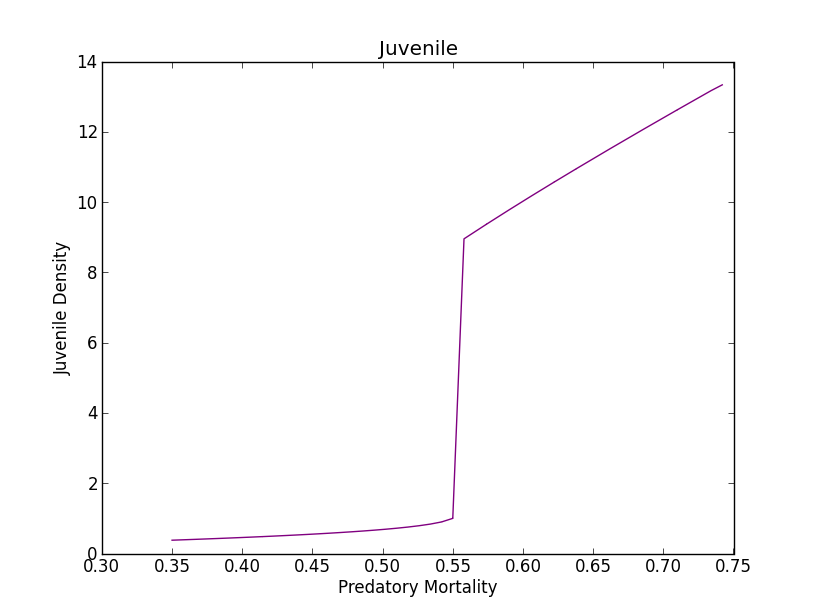
\includegraphics[width=\linewidth]{juvenile_bifurcation.png}
  \caption{Juvenile population density ($J$) v. increasing values for predator mortality ($\mu_P$)}
\endminipage\hfill
\minipage{0.5\textwidth}
  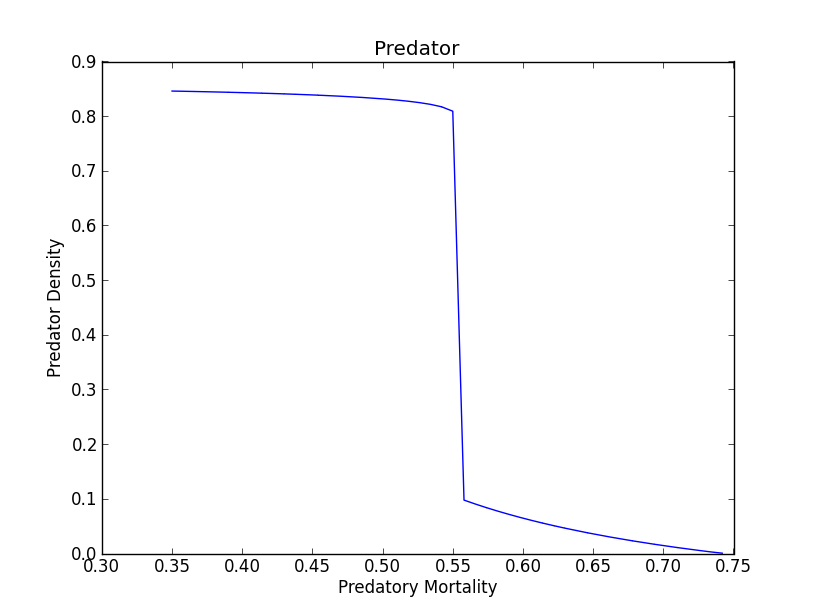
\includegraphics[width=\linewidth]{predator_bifurcation.png}
  \caption{Predator population density ($P$) v. increasing values for predator mortality ($\mu_P$)}
\endminipage\hfill
\end{centering}
\end{figure}
\FloatBarrier

This system exhibits a classic fold bifurcation \cite{Scheffer2001} in the parameter space of the predator mortality rate ($\mu_P$) measured against the various population densities. There is a sudden, discontinuous shift in the system at $\mu_P \approx 0.553$. More precisely, between the bifurcation points $T_1(\mu_ P<0.553)$ and $T_2 (\mu_ P<0.435)$ the system is bistable with an unstable intermediate saddle-node. This instability is illustrated in Fig. 4:

\begin{figure}[!htb]
\centerline{
\minipage{0.7\textwidth}
  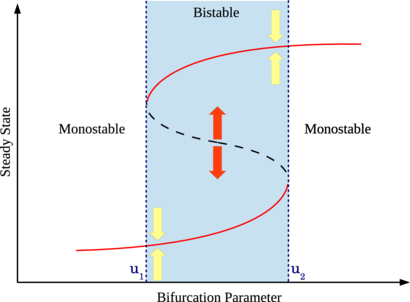
\includegraphics[width=\linewidth]{foldbif.png}
  \caption{An example of a system with two stable states and an unstable intermediate saddle-node.} 
\endminipage
}
\end{figure}
\FloatBarrier

In short, we see a catastrophic collapse in the predator density due to increasing predator mortality. In a real-world context, this increasing pressure on the predator population via an increase in the intrinsic mortality rate could be thought of as increasing pressure due to over-harvesting (in a coupled human-environmental system context), the impact of new pathogens, or environmental degradation. What's most interesting, however, is that this sudden shift between predator-free and predator-inhabited regimes has no impact on the adult densities ($A$):

\begin{figure}[!htb]
\centerline{
\minipage{0.7\textwidth}
  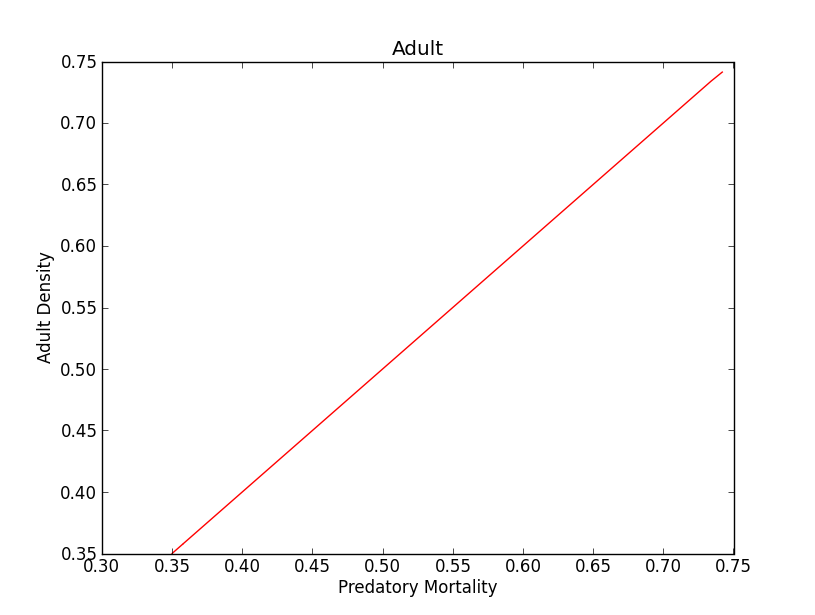
\includegraphics[width=\linewidth]{adult_bifurcation.png}
  \caption{Adult population density ($A$) v. increasing values for predator mortality ($\mu_P$). Note that no change in $A$ is observed at the parameter value $\mu_P \approx 0.553$ at which the juvenile population density shows a sudden transition.}
\endminipage
}
\end{figure}
\FloatBarrier


%-------------------------------------------------
% The Alternative Stable States of the ODE Model
%-------------------------------------------------
\subsection{The Alternative Stable States of the ODE Model}
As I have shown, there are two separate stable equilibria in this model: predator-free ($P=0$) and predator-present ($P>0$). Below $\mu_P \approx 0.553$, we see an equilibrium evolve which has steady, non-zero population densities of predators, adults, and juveniles. Above $\mu_P \approx 0.553$, we see an equilibrium state in which predators are no longer found. If we solve for the coupled ordinary differential equation at values of $\mu_P$ that are firmly within each state, we can graphically see the population densities approach equilibrium. When $\mu_P=0.7$, the predators die out, as shown in Figure 6.

\begin{figure}[!htb]
\centerline{
\minipage{0.7\textwidth}
  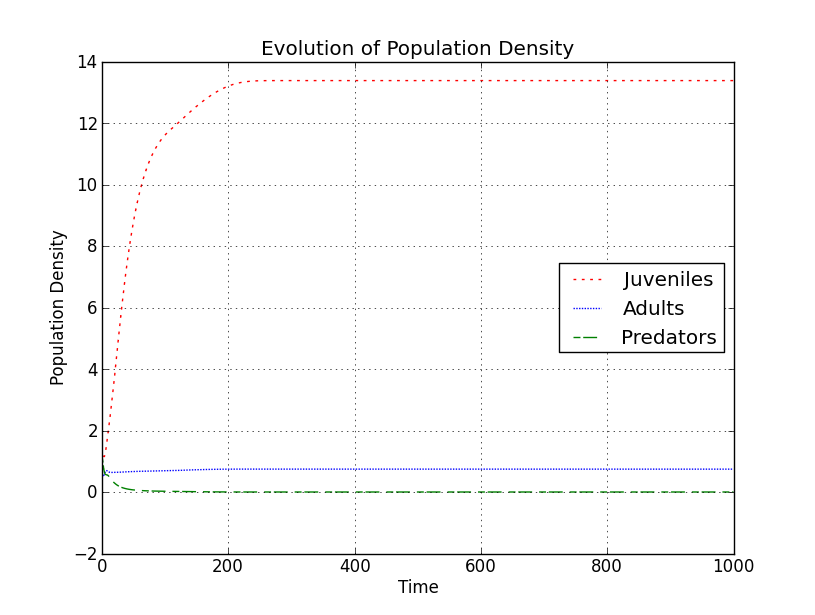
\includegraphics[width=\linewidth]{population_density_uP_high.png}
  \caption{Population densities over time for juveniles, adults, and predators, with $\mu_P = 0.7$.} 
\endminipage
}
\end{figure}
\FloatBarrier

Figure 6 shows how the population densities of juveniles, adults, and predators evolve towards an equilibrium state in which there is a very high density of juvenile prey and a low density of adult prey in the environment, with predators quickly dying out. 
\begin{figure}[!htb]
\centerline{
\begin{centering}
\minipage{0.7\textwidth}
  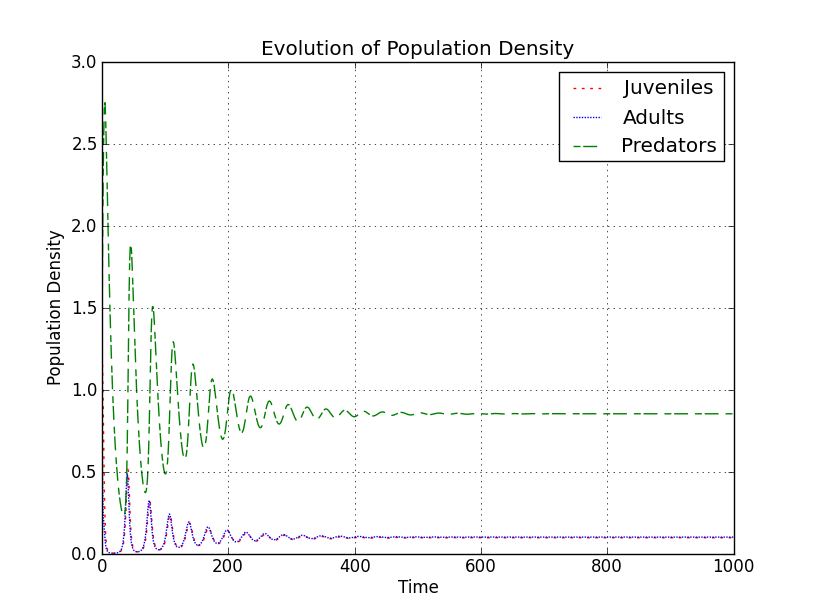
\includegraphics[width=\linewidth]{population_density_uP_low.png}
  \caption{Population densities over time for juveniles, adults, and predators, with $\mu_P = 0.1$.} 
\endminipage
\end{centering}
}
\end{figure}
\FloatBarrier

On the other hand, if $\mu_P = 0.1$, the predators do not die out. This is shown in Fig. 7, where we see an initial period of oscillatory behavior before the various populations settle into steady densities. The purpose of our study is, however, to see if there is any form of EWS present in the time-series of our model as it approaches and crosses the threshold separating the two steady states. To see how the behavior of the model changes during this transition in general, Figure 8 shows the transition of the model starting from $\mu_P = 0.100$ and increasing by $0.001$ at every time step\footnote{A clarifying statement regarding the phrase "time-step" is needed. We first solve the ordinary differential equations to find a current population density vector, $X_1$. Then, utilizing these new population density values, solve the ordinary differential equations once more to obtain a new set of population densities, vector $X_2$. This iterative process between $X_1$ and $X_2$  is one "time-step". To model a continuous function (such as an ODE), each "time-step" contains a number of user-specified intermediate values which "bridge" the possibly discrete values between "time-steps". For this paper, we have used 10 intermediate values (or $\Delta t = 10$) between each "time-step".} until the bifurcation point ($\mu_P \approx 0.553$) is surpassed:

\begin{figure}[!htb]
\centerline{
\begin{centering}
\minipage{0.7\textwidth}
  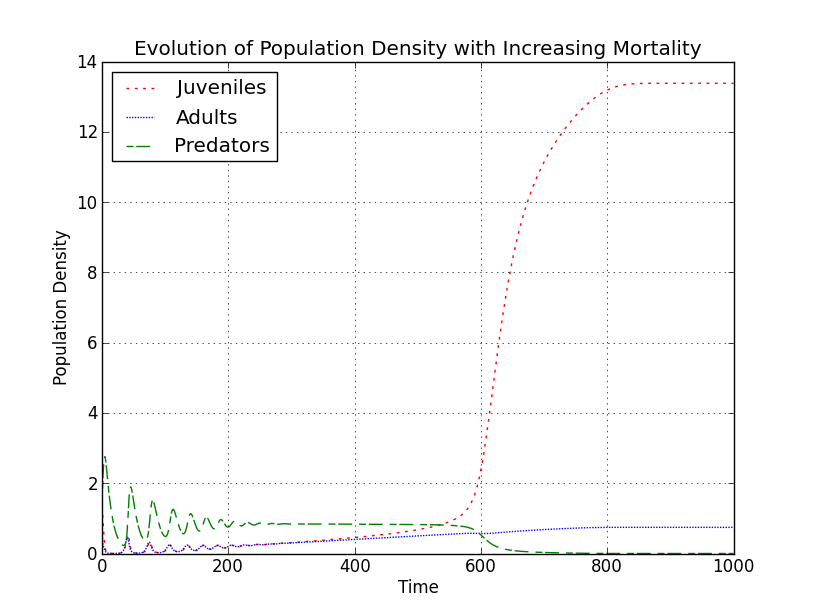
\includegraphics[width=\linewidth]{population_density_with_increasing_uP.png}
  \caption{Population densities over time of juveniles, adults, and predators, with an increasing value for $\mu_P$ (from $\mu_P = 0.001$ to $\mu_P = 0.999$)} 
\endminipage
\end{centering}
}
\end{figure}
\FloatBarrier
Fig. 8 clearly displays the transition between a predator-inhabited and predator-free environment. If we apply our earlier mentioned suite of early warning signals, will we observe any potential signs of the impending transition before it occurs? To check, we will utilize the package  \texttt{earlywarnings} in the R programming language to analyze the various early warning signals that may be present in the solutions to our set of coupled ordinary differential equations ( Eq. (7-9)). However, before I analyze my ODE model, it may be useful to examine a dataset that has known EWS. To do so, I will utilize the \texttt{foldbif} dataset from the \texttt{earlywarnings} package as an educational example and future reference. The \texttt{earlywarnings} package is an open source suite of statistical methods as introduced in \cite{Dakos2012} used to calculate the various theorized early warning signals discussed in this work.


%-------------------------------------------------
% Early warning signals - example
%-------------------------------------------------
\subsection{An Example of Early Warning Signals}

I will utilize the \texttt{foldbif} dataset (included in the \texttt{earlywarnings} package in R) to show what our early warning signals look like in a dataset that clearly shows critical slowing down. The time-series output of 'foldbif' looks like this:


\begin{figure}[!htb]
\centerline{
\begin{centering}
\minipage{0.7\textwidth}
  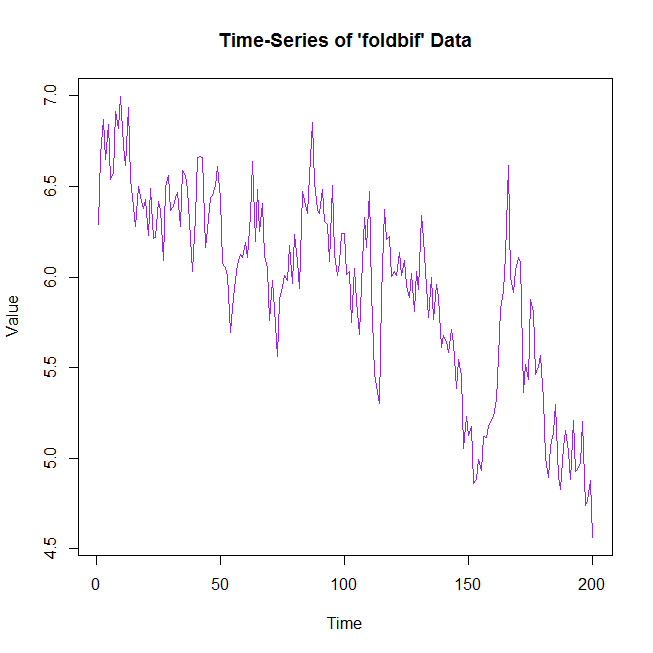
\includegraphics[width=\linewidth]{foldbifdata.png}
  \caption{Time-series plot of \texttt{foldbif} dataset.} 
\endminipage
\end{centering}
}
\end{figure}
\FloatBarrier

Visually, we can see that this dataset is exhibiting a general downward trend. It also \emph{seems} as though the dataset shows increasingly slow recovery from shocks, but this is difficult to intuit from a simple time-series plot. However, what we cannot visually see is the early warning signals that may be present in the data analysis. Let's examine the early warning signals (EWS) as output by the \texttt{generic\textunderscore ews()} function in R.

\begin{figure}[!htb]
\centerline{
\begin{centering}
\minipage{\textwidth}
  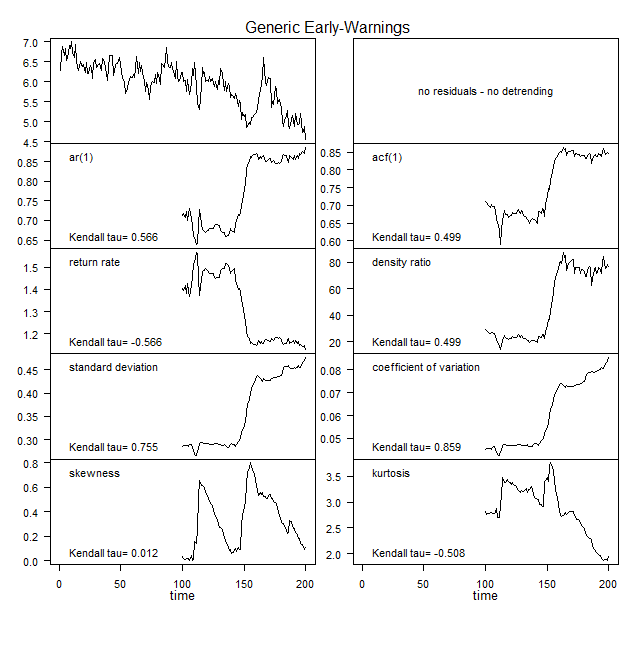
\includegraphics[width=\linewidth]{foldbifews.png}
  \caption{Output from "Early Warning Signals Tool-kit" in R for the \texttt{foldbif} dataset}
\endminipage
\end{centering}
}
\end{figure}
\FloatBarrier

Fig. 10 is the primary output from the Early Warning Signals tool-kit. The top-left window is simply a repetition of the time-series values for the dataset (\texttt{foldbif}). The adjacent window displays that we have not applied any detrending methods to the dataset. The window labeled "ar(1)" displays a plot of the autocorrelation-at-lag-1. The window "acf(1)" is the a plot of the autocorrelation-at-first-lag (which we will subsequently ignore). The "return rate" window is a plot of the return rate of the dataset, estimated as 1- ar(1). The window "density ratio" is the plot of the power spectrum of the data as the ratio of low frequencies over high frequencies. The windows "standard deviation", "coefficient of variation", "skewness", and "kurtosis" are all self-explanatory. Each of these windows will be covered in further detail in subsequent analysis. What is important to note is the general trend of the EWS: ar(1), standard deviation, the coefficient of variation, and the density ratio are all increasing, much as our understanding of critical slowing down and EWS predicts. We are also seeing drastic changes in skewness and some ambiguous measures of kurtosis \footnote{The expected EWS for skewness and kurtosis are far more pronounced if we apply Gaussian or linear detrending to the dataset. For the sake of brevity, I have left such issues of detrending out of the subsequent analysis. It is worth noting, however, the detrending may play a pivotal role in understanding certain forms of EWS in datasets.}.  What's most important is that we see these trends \emph{before} the critical transition takes place (which occurs at $t\approx 150$). After this point, though the system shows a momentary large gain, it quickly (in relative terms) loses ground and decreases at a faster rate. Therefore, if we wanted to be able to forecast the projected system behavior, the ability to have warnings of such sudden shifts would be of tremendous value. Now let's move on to the EWS present in our predator, adult, and juvenile population densities from the ODE. 

%-------------------------------------------------
% Early warning signals - predator
%-------------------------------------------------
\subsection{Early Warning Signals in Predator Density}

The output of our Early Warning Signals Tool-kit for the predator population density is shown in Fig. 11. 
\begin{figure}[!htb]
\centerline{
\begin{centering}
\minipage{\textwidth}
  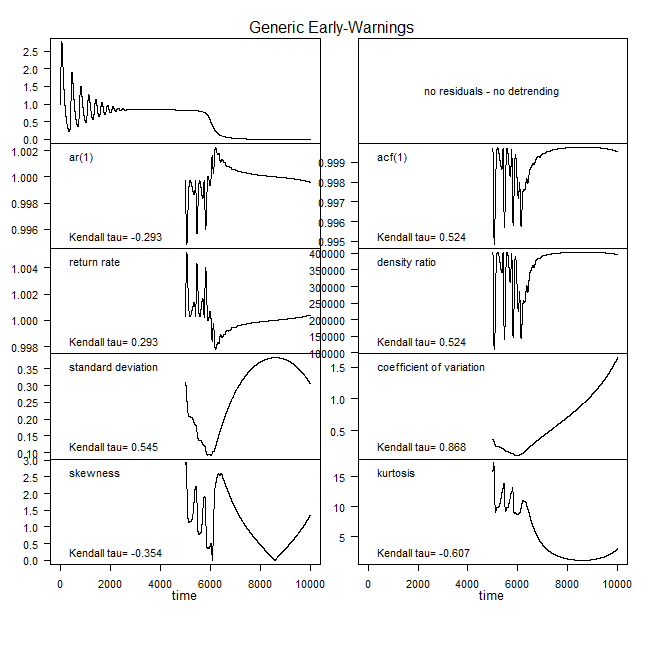
\includegraphics[width=\linewidth]{generic_ews_pred_winsize_50.png}
  \caption{Output from "Early Warning Signals Tool-kit" in R for the predator density ($P$) from the ODE model.  (\texttt{winsize = 50})} 
\endminipage
\end{centering}
}
\end{figure}
\FloatBarrier
It is important to note is that the expected behavior of our early warning signals is not present, nor are the signals that are present entirely clear. We must also note why the EWS only provides values for $t>500$. The \texttt{earlywarnings} packages computes all of the EWS within a rolling statistical window that is equal to fifty percent of the time-series. Therefore, it will only begin to compute values at the "halfway" point in the time-series. \footnote{A special note on the difference in time-scales. The reader may have noticed a discrepancy between the time-scales on the previous plots in this paper (generated in Python via NumPy) and those being offered here (generated in R) . The algorithm used to solve for the coupled ordinary differential equations in NumPy will return the number of user-specified intermediate values for each time-step [as mentioned before, our $\Delta t=10$, so there are 10 values between $t=0$ and $t=1$]. This is a by-product of the algorithm solving the ODE to provide a continuous solution. The \texttt{plot()} function in R utilized the raw output file from this process, which \emph{actually} includes 10,000 raw data points. The discrepancy is therefore one of labeling and not data misrepresentation.} We will examine each closely.\footnote{A few words on the Kendall tau statistic. The Kendall tau statistic ($\tau$) provides the nonparametric correlation measure between two variables. In short: the Kendall tau statistic is just the number of observation pairs which move in the same direction, minus the number of observation pairs moving in the opposite direction, divided by the number of possible pairs. Hence, the more numbers of pairs of observations (for example, between values in our time series and ar(1) values) that are moving in the same direction, the higher the $\tau$. } 

\begin{figure}[!htb]
\begin{centering}
\minipage{0.5\textwidth}
  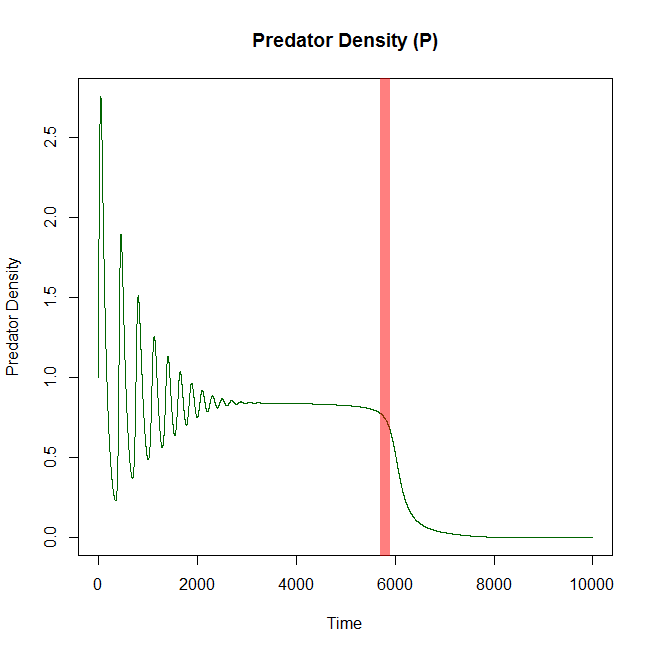
\includegraphics[width=\linewidth]{generic_ews_pred_ts_windsize_50.png}
  \caption{Predator density ($P$)} 
\endminipage\hfill
\minipage{0.5\textwidth}
  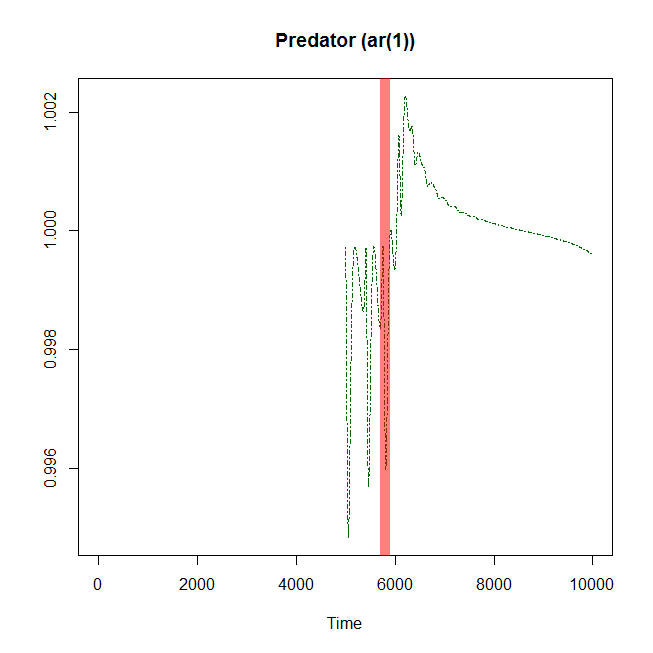
\includegraphics[width=\linewidth]{generic_ews_pred_ts_ar1_windsize_50.png}
  \caption{ar(1) of predator density ($P$)}
\endminipage\hfill
\end{centering}
\end{figure}
\FloatBarrier

Figures 12 and 13 have simply isolated the first window (the predator density $P$ over time) and the third window (the values of ar(1) for $P$ over time) from the large set of plots above. I have also added an opaque red line to show the approximate location of the bifurcation point in the time-series (at which $\mu_P \approx 0.553$). As we can see, the output of the ar(1) process does not follow the trend that our theory predicts. Instead of seeing a consistently increasing value for our autocorrelation function as it nears the critical transition, we instead see large fluctuations without an overall trend. In fact, we only observe a drastic increase in autocorrelation \emph{after} the critical transition has taken place. This may give us room for pause. What of the other early warning signals, such as the coefficient of variation and standard deviation?

\begin{figure}[!htb]
\begin{centering}
\minipage{0.5\textwidth}
  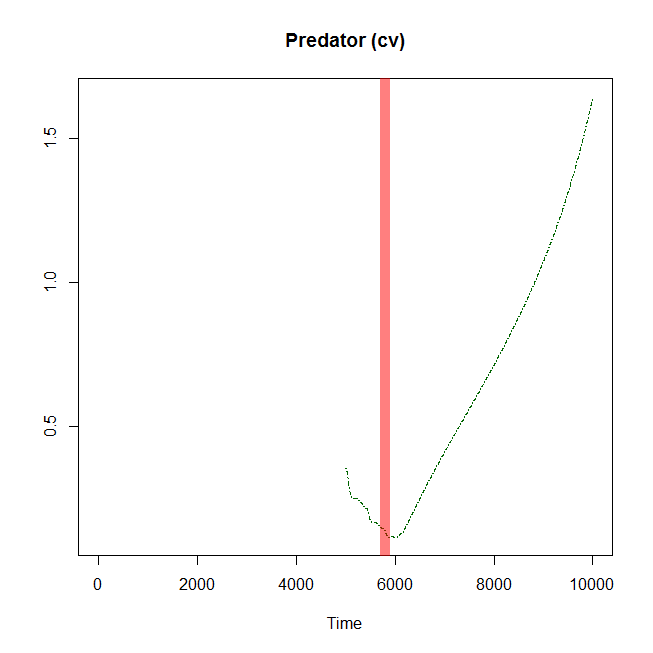
\includegraphics[width=\linewidth]{generic_ews_pred_ts_cv_windsize_50.png}
  \caption{Coefficient of variation of predator density ($P$)} 
\endminipage\hfill
\minipage{0.5\textwidth}
  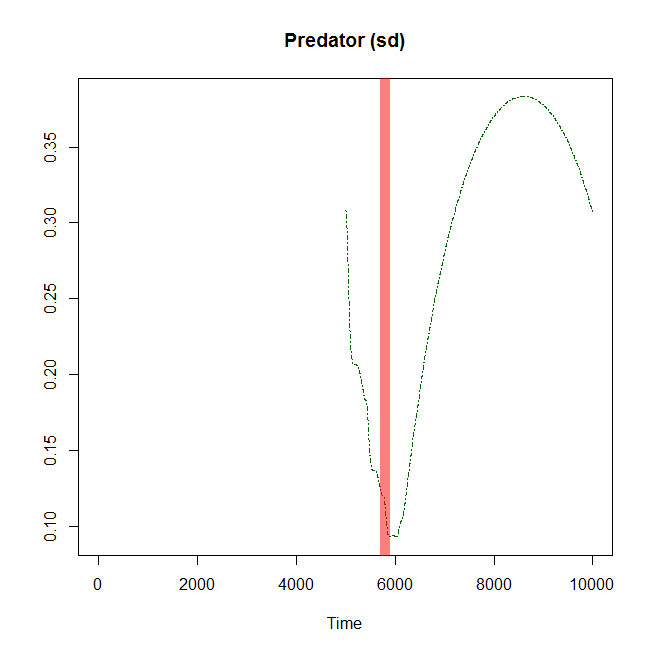
\includegraphics[width=\linewidth]{generic_ews_pred_ts_sd_windsize_50.png}
  \caption{Standard deviation (sd) of predator density ($P$)}
\endminipage\hfill
\end{centering}
\end{figure}
\FloatBarrier

Figures 14 and 15 are equally misleading. We expect variance to be increasing as we near the bifurcation point (shown as the red bar, where $\mu_P \approx 0.553$), yet here we can visually see that it is in fact \emph{decreasing} before this point. Again, much as with our values for the ar(1) process, we see that the expected increases in both the coefficient of variation and standard deviation occur only after the critical transition has been passed through. It is much the same story for skewness and kurtosis:

\begin{figure}[!htb]
\begin{centering}
\minipage{0.5\textwidth}
  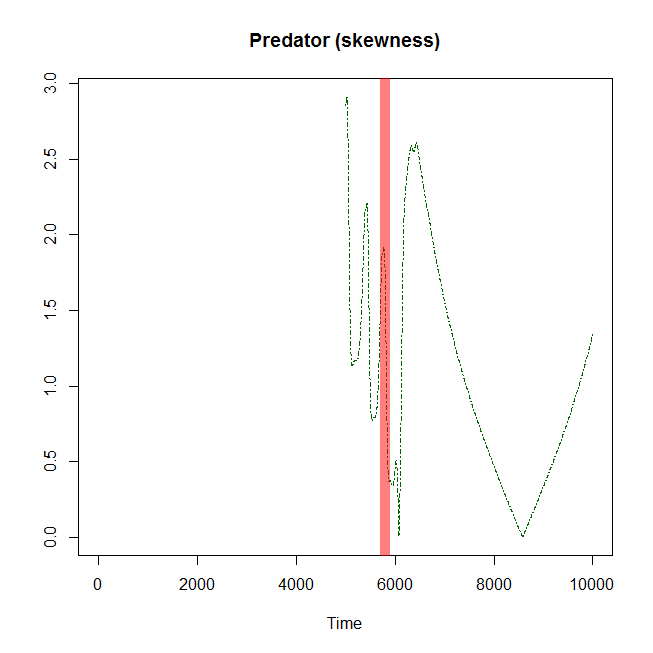
\includegraphics[width=\linewidth]{generic_ews_pred_ts_sk_windsize_50.png}
  \caption{Skewness predator density ($P$)} 
\endminipage\hfill
\minipage{0.5\textwidth}
  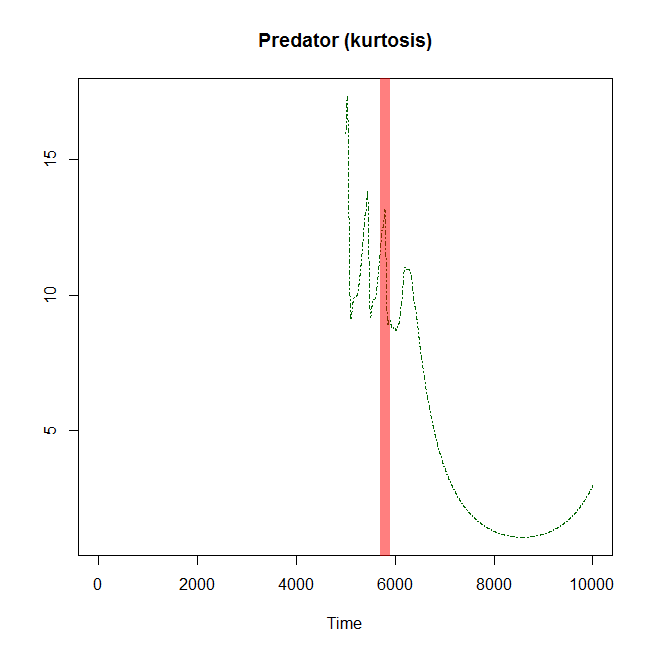
\includegraphics[width=\linewidth]{generic_ews_pred_ts_kurt_windsize_50.png}
  \caption{Kurtosis of predator density ($P$)}
\endminipage\hfill
\end{centering}
\end{figure}
\FloatBarrier
It is worth noting that there is a weak early warning signal present in the skewness measure, as we are measuring absolute \emph{change} in the skewness as opposed to an increase or decrease, but this change is hidden by the rapid variations directly preceding the bifurcation point. This signal is not present in the measure of kurtosis in Fig. 17.

\begin{figure}[!htb]
\centerline{
\begin{centering}
\minipage{0.7\textwidth}
  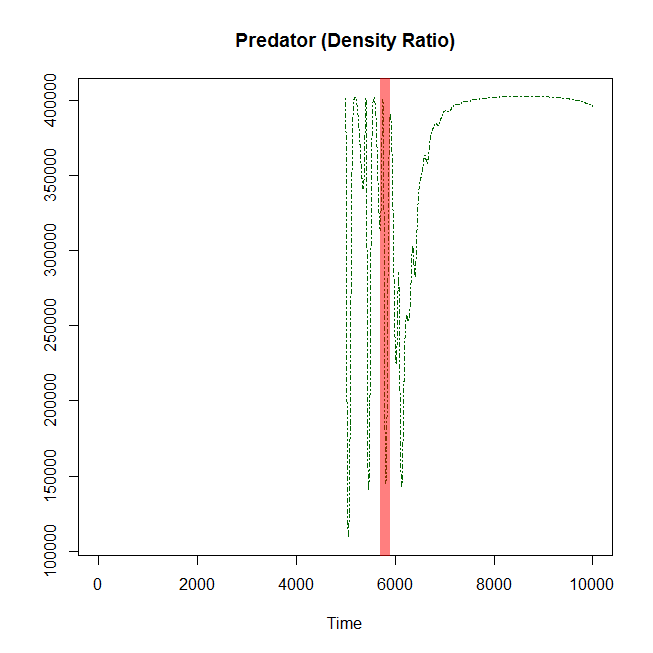
\includegraphics[width=\linewidth]{generic_ews_pred_ts_spec_density_windsize_50.png}
  \caption{Spectral density ratio of predator density ($P$)} 
\endminipage
\end{centering}
}
\end{figure}
\FloatBarrier

Finally, we can take a look at the spectral properties of our time-series by examining Fig. 18. As I have referenced above, one of the ways in which to diagnose the phenomenon of spectral reddening is to observe an increase in the spectral density ratio. This implies a switch in the spectral density between a state dominated by high-frequency process to one dominated by low-frequency processes (which may imply critical slowing down). We calculate the spectral density ratio as the ratio between spectral densities at a frequency of 0.05 (low frequency processes) and densities at the frequency of 0.5 (high frequency processes). Thus, a higher value for our spectral density ratio implies spectral reddening. What we see in Figure 19 is therefore somewhat confusing. Much as we noticed in the ar(1) values, we see large negative fluctuation around a stable state as we approach the bifurcation point. Again, we only see the signature marks of spectral-reddening after the critical transition has occurred. \\

The difficulties thus far encountered in discovering early warning signals in the predator density over time pose not just difficult theoretical questions but also may be serious problems in terms of application. Predator species within ecosystems tend to be the most economically valuable (especially in marine ecosystems). If the goal of a particular conservation scheme is to \emph{prevent} the collapse of a predator species, it is important to know that the potential early warning signals of a critical transition may be absent in the time-series data that represents that specific species density. \\

This is, however, not a time for despair! Perhaps it is in the adult prey that we find our early warning signals for a critical transition. After all, the predator species wholly subsists on the adults as a food source. It would therefore be quite reasonable to suspect that perturbations in the predator species may be detected in the adult population density $A$.  \\

%-------------------------------------------------
% Early warning signals - adults - window size 50 
%-------------------------------------------------
\subsection{Early Warning Signals in Adult Density}

We again begin our analysis by observing the output from the Early Warning Signals tool-kit. Figure 19 once again displays both the original time-series values values for our adult population density and the relevant statistical metrics which have been theorized to provide early warning signals for critical transitions \footnote{Of note is the slight plateau in the time-series for $A$ present in Fig. 19 that is not discernible in Figure 6.}. Though this figure visually provides all of the information that we need, it may once more be useful to progress through the various plots one by one.

\begin{figure}[!htb]
\centerline{
\begin{centering}
\minipage{\textwidth}
  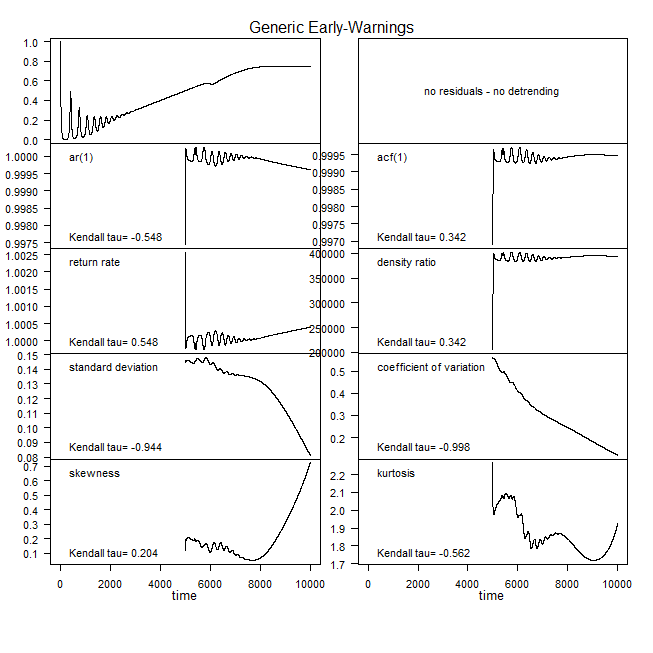
\includegraphics[width=\linewidth]{generic_ews_adult_windsize_50.png}
  \caption{Output from "Early Warning Signals Tool-kit" in R for the adult density ($A$) from the ODE model.  (\texttt{winsize = 50})} 
\endminipage
\end{centering}
}
\end{figure}
\FloatBarrier

Again, let's examine each of the relevant figures more closely. Figure 20 displays the ar(1) values within the rolling window. Once more, we see fluctuations around a stationary point (though not of the magnitude of the fluctuations present in the ar(1) for $P$) and a gradual trend of oscillatory decay after the point of the critical transition. Thus, there is no clear early warning signal present. This is the same for Fig. 21. Here, the coefficient of variation is decidedly \emph{decreasing} across the entirety of the rolling window. This stands in direct contrast to what the theoretical support for early warning signals would predict. 

\begin{figure}[!htb]
\minipage{0.5\textwidth}
  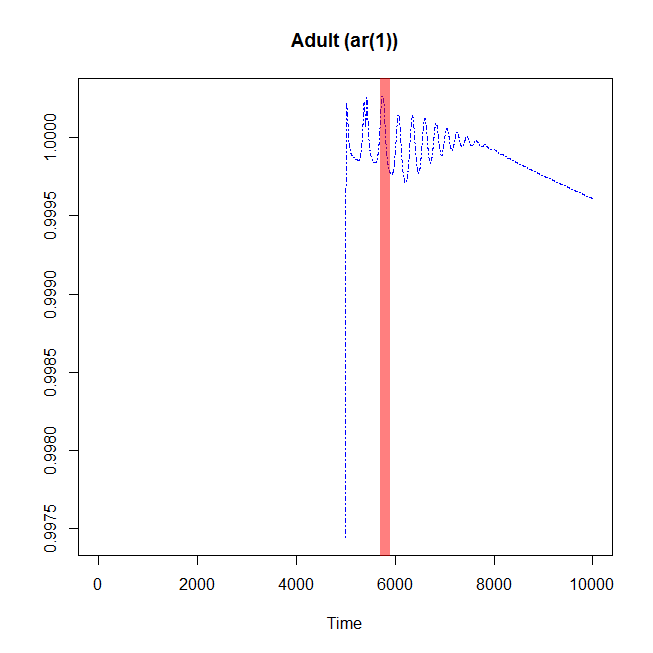
\includegraphics[width=\linewidth]{generic_ews_adult_ts_ar1_windsize_50.png}
  \caption{ar(1) of adult density ($A$)} 
\endminipage\hfill
\minipage{0.5\textwidth}
  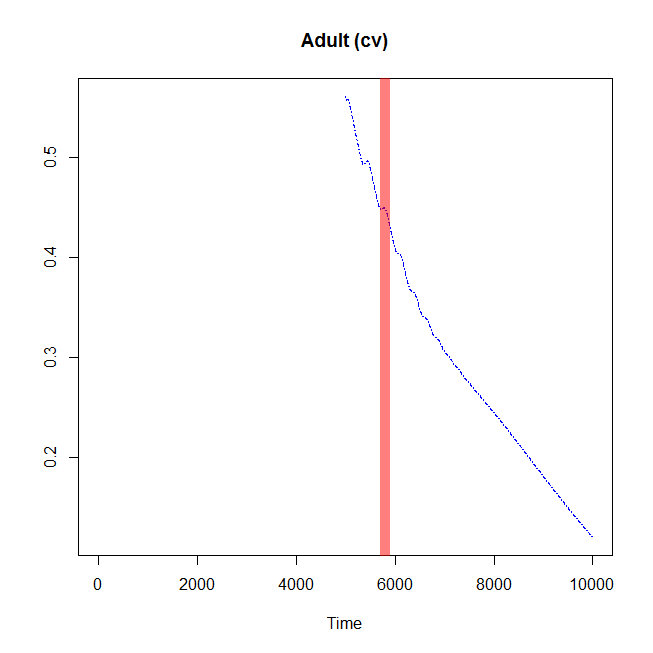
\includegraphics[width=\linewidth]{generic_ews_adult_ts_cv_windsize_50.png}
  \caption{Coefficient of variation of adult density ($A$)}
\endminipage\hfill
\end{figure}
\FloatBarrier

The same holds true for standard deviation and skewness, as found in Figs. 22 and 23. 

\begin{figure}[!htb]
\minipage{0.5\textwidth}
  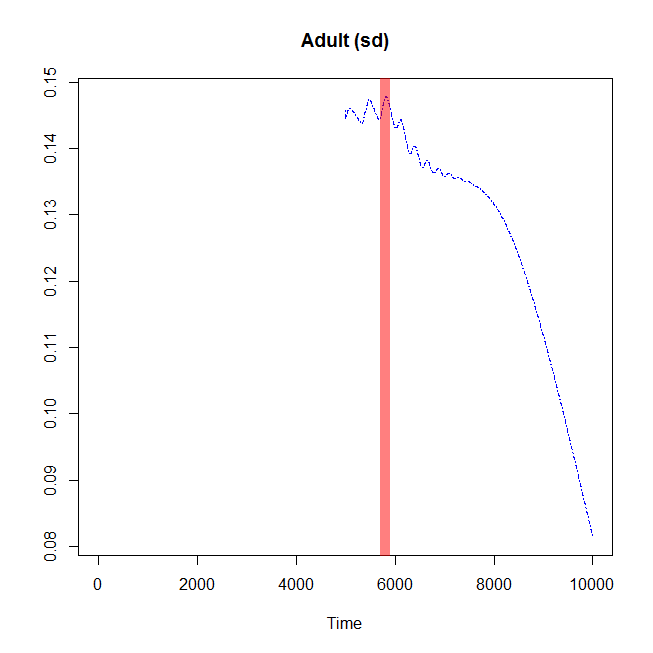
\includegraphics[width=\linewidth]{generic_ews_adult_ts_sd_windsize_50.png}
  \caption{Standard deviation of adult density ($A$)} 
\endminipage\hfill
\minipage{0.5\textwidth}
  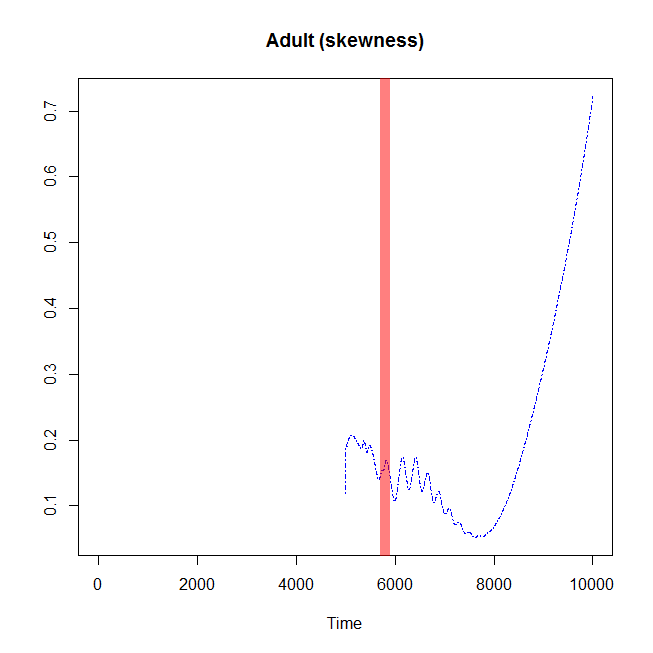
\includegraphics[width=\linewidth]{generic_ews_adult_ts_sk_windsize_50.png}
  \caption{Skewness of adult density ($A$)}
\endminipage\hfill
\end{figure}
\FloatBarrier

Perhaps something will appear in the measures of kurtosis or the spectral density ratio?


\begin{figure}[!htb]
\begin{centering}
\minipage{0.5\textwidth}
  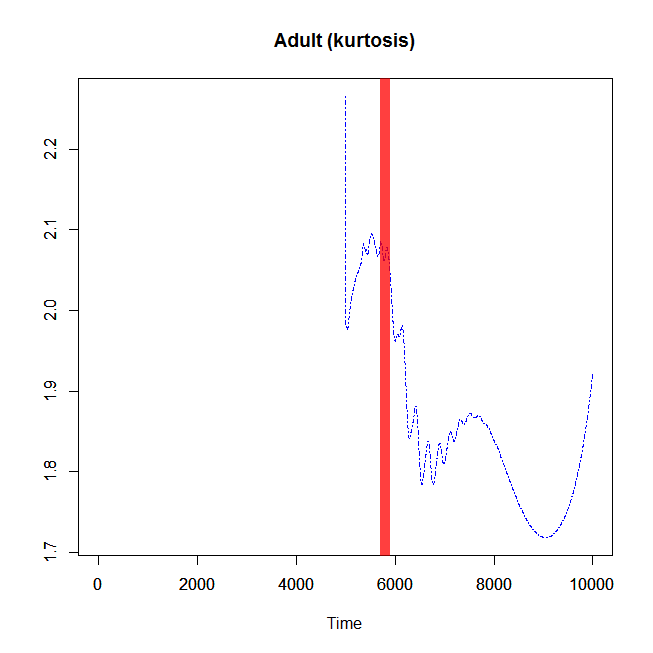
\includegraphics[width=\linewidth]{generic_ews_adult_ts_kurt_windsize_50.png}
  \caption{Kurtosis of adult density ($A$)} 
\endminipage\hfill
\minipage{0.5\textwidth}
  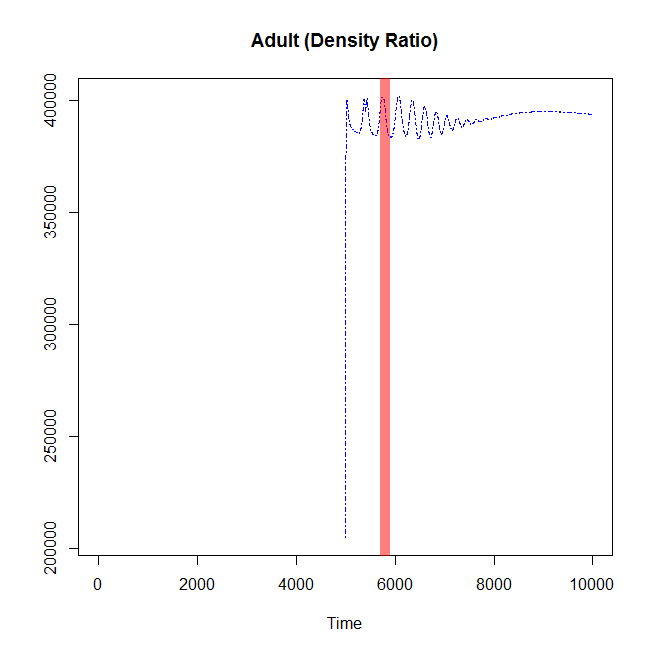
\includegraphics[width=\linewidth]{generic_ews_adult_ts_spec_density_windsize_50.png}
  \caption{Spectral density ratio of adult density ($A$)}
\endminipage\hfill
\end{centering}
\end{figure}
\FloatBarrier

Here again we are faced with the same problem as in the predator population. Our spectral density ratio values exhibit decaying oscillatory behavior (which is, coincidentally, also what we find in the time-series values of $A$ itself) and not the spectral reddening that we expect. \\

In conclusion, there are no early warning signals present in the time-series of $A$. Though disconcerting, this is not entirely unexpected, as the relationship we derived in Eq. 16 explicitly connected predator mortality ($\mu_P$) to juvenile population density ($J$), not adult population density ($A$). Perhaps the critical transition will exhibit early warning signals in the juvenile population density time-series. 
%-------------------------------------------------
% Early warning signals - juvenile - window size 50 
%-------------------------------------------------
\subsection{Early Warning Signals in Juvenile Density}

\begin{figure}[!htb]
\centerline{
\begin{centering}
\minipage{\textwidth}
  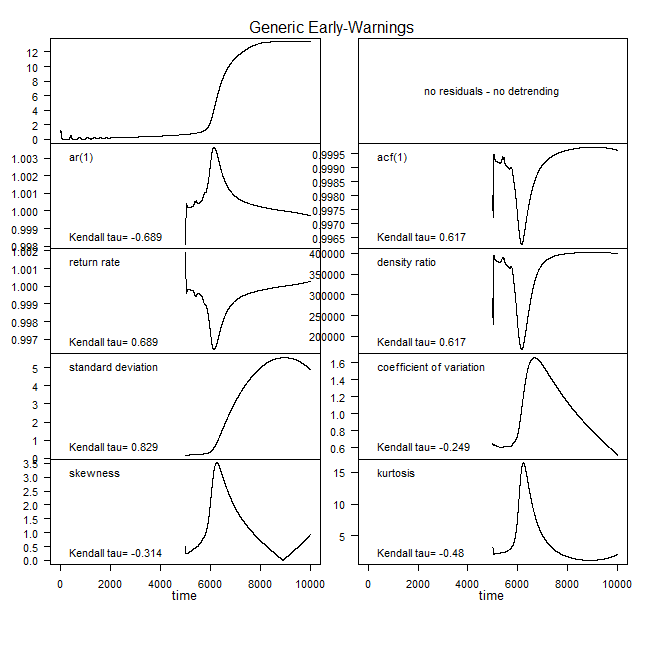
\includegraphics[width=\linewidth]{generic_ews_juv_windsize_50.png}
  \caption{Output from "Early Warning Signals Tool-kit" in R for the juvenile density ($J$) from the ODE modell.  (\texttt{winsize = 50})} 
\endminipage
\end{centering}
}
\end{figure}
\FloatBarrier

Once more, let us examine each of the output graphs in closer detail.

\begin{figure}[!htb]
\begin{centering}
\minipage{0.5\textwidth}
  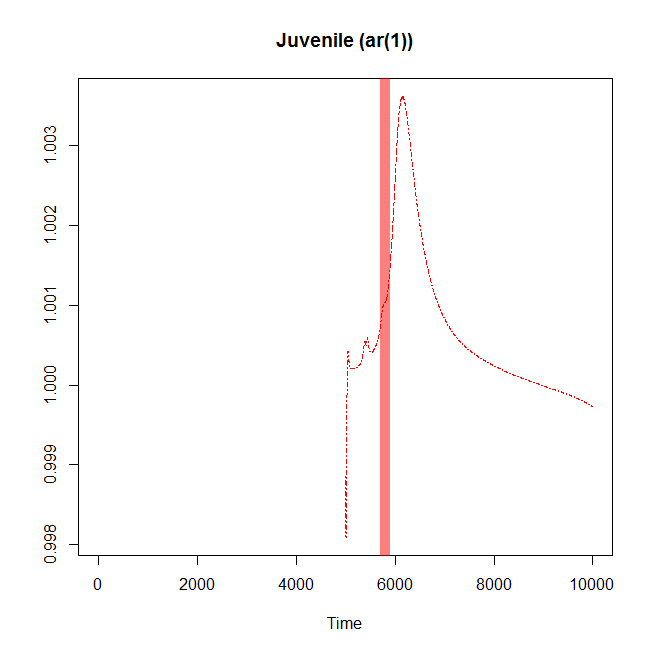
\includegraphics[width=\linewidth]{generic_ews_juv_ts_ar1_windsize_50.png}
  \caption{ar(1) of juvenile density ($J$)} 
\endminipage\hfill
\minipage{0.5\textwidth}
  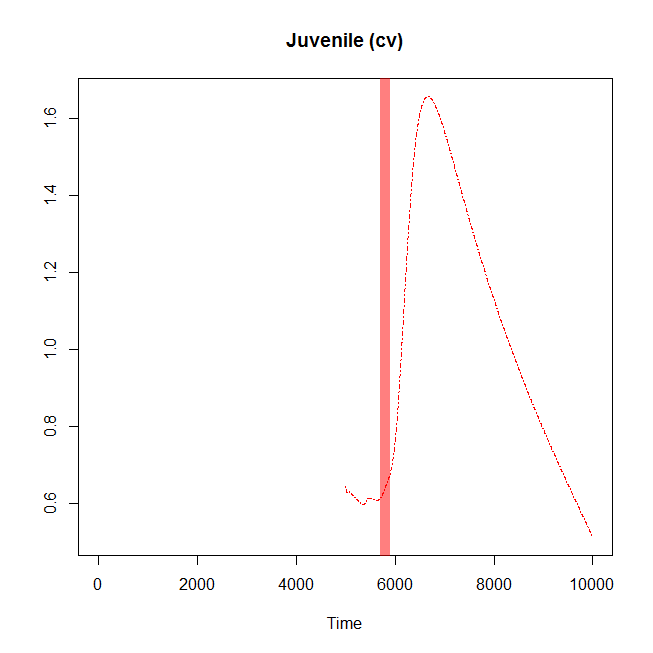
\includegraphics[width=\linewidth]{generic_ews_juv_ts_cv_windsize_50.png}
  \caption{Coefficient of variation  of juvenile density ($J$)}
\endminipage\hfill
\end{centering}
\end{figure}
\FloatBarrier

Here, we see a promising increase in the ar(1) values of our time-series in Fig. 27. Once again, however, the bulk of the increase takes place after the bifurcation point has been passed through. The same is true for our measurement of the coefficient of variation as shown in Fig. 28.

\begin{figure}[!htb]
\minipage{0.5\textwidth}
  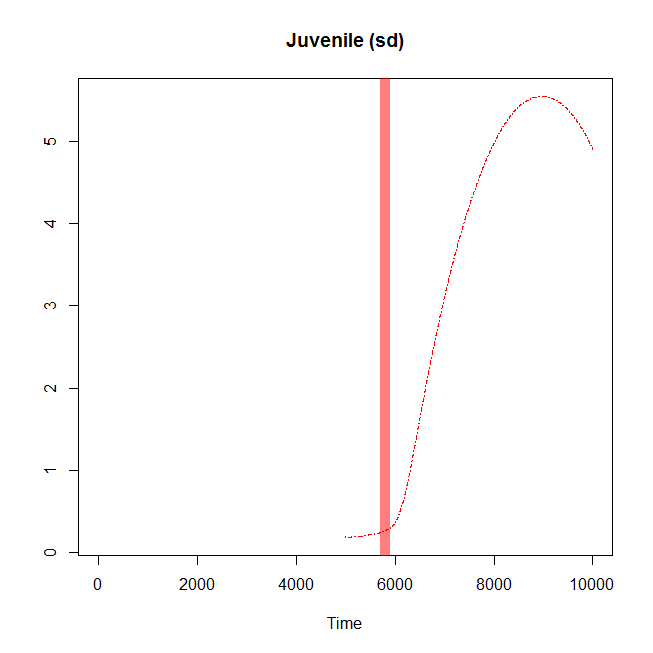
\includegraphics[width=\linewidth]{generic_ews_juv_ts_sd_windsize_50.png}
  \caption{Standard deviation of juvenile density ($J$)} 
\endminipage\hfill
\minipage{0.5\textwidth}
  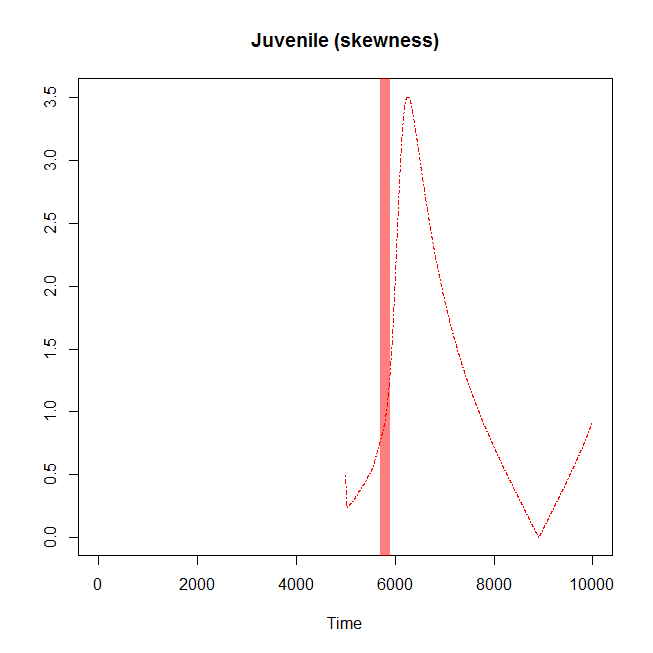
\includegraphics[width=\linewidth]{generic_ews_juv_ts_sk_windsize_50.png}
  \caption{Skewness of juvenile density ($J$)}
\endminipage\hfill
\end{figure}
\FloatBarrier

We once again see a "silent" catastrophe when measuring standard deviation (Fig. 29), skewness (Fig. 30) and kurtosis (Fig. 31). But what of the spectral density ratio in Fig. 32?


\begin{figure}[!htb]
\begin{centering}
\minipage{0.5\textwidth}
  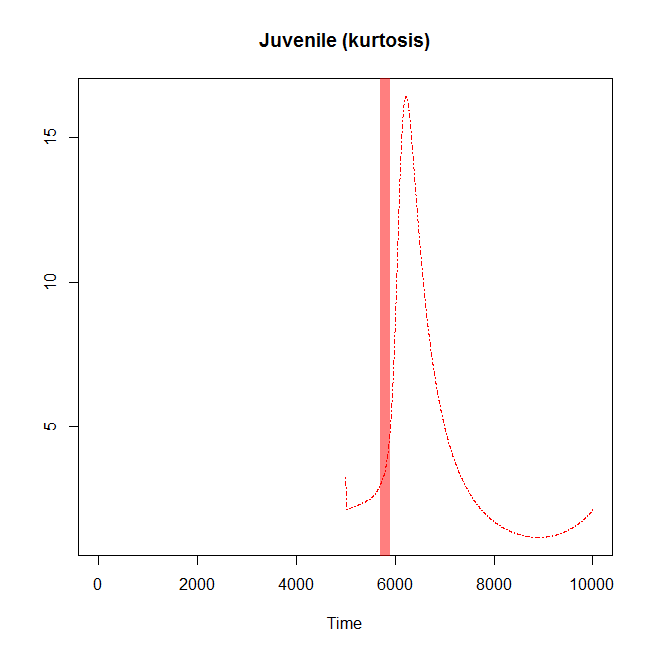
\includegraphics[width=\linewidth]{generic_ews_juv_ts_kurt_windsize_50.png}
  \caption{Kurtosis of juvenile density ($J$)} 
\endminipage\hfill
\minipage{0.5\textwidth}
  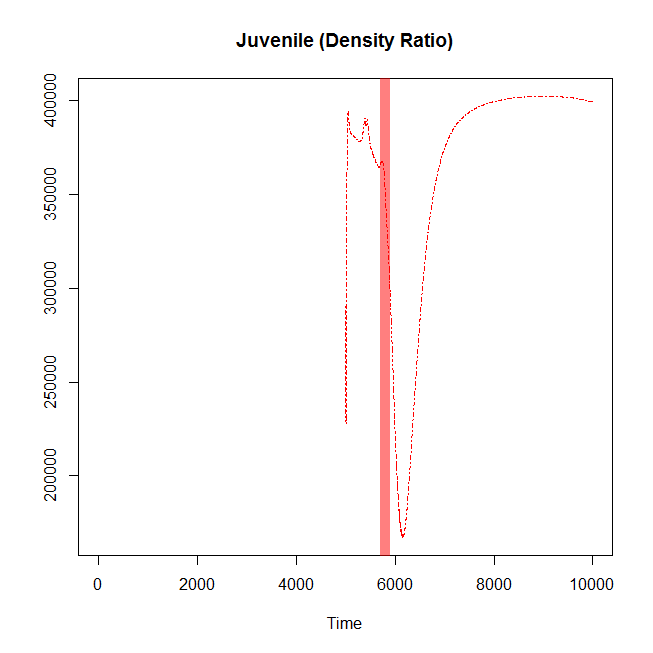
\includegraphics[width=\linewidth]{generic_ews_juv_ts_spec_density_windsize_50.png}
  \caption{Spectral density ratio of juvenile density ($J$)}
\endminipage\hfill
\end{centering}
\end{figure}
\FloatBarrier

Figure 32 shows a high spectral density (meaning an observation of spectral reddening) just prior to the critical transition, but rapidly decreases as the transition is passed through. Though this small (but promising) early warning signal seems to exist in the spectral density ratio, our general findings thus far find us in agreement with \cite{Boerlijst2013}: the generic early warning signals used to detect critical transitions in this model are mostly absent. This is in many ways to be expected of a system of ordinary differential equations without a noise term: without random fluctuations, there may be no variations to capture within the statistical rolling window except those which occur at the bifurcation point, leading to spurious findings.\\

However, there is room for improvement in our ODE model specifications that may allow for the possibility of early warning signals to be more readily detected. Many model specifications of ecological systems invoke various degrees of stochastic forcing (or noise) to perturb state variables, usually intended to represent (in a generic way) difficult to quantify random environmental shocks. Such disturbances may actually aid in the discovery of early warning signals, as the addition of random elements into the system may make the discovery of critical transitions simpler by amplifying statistical features of the time-series. We must therefore explore the possibilities of adding stochastic elements to our coupled set of ordinary differential equations. For the sake of brevity, we will focus on the two most common forms of additive noise in ecological models: independent (also known as white) noise and autocorrelated noise-- also known as pink or $\dfrac{1}{f}$ noise. 


%-------------------------------------------------
% Early warning signals in the equation-based model with independent noise
%-------------------------------------------------
\subsection{The ODE Model with Independent (White) Noise}

We again begin with the ODE model:
\begin{align}
	& \dfrac{dJ}{dt} = bA - \dfrac{J}{(1+J^2)} - \mu_JJ\\
	& \dfrac{dA}{dt} = \dfrac{J}{(1+J^2)} - APc - \mu_AA\\
	& \dfrac{dP}{dt} = P(cA - \mu_p)
\end{align}
However, we will now add a white-noise term, $\omega$, to the predator mortality rate. This term is a Gaussian noise process with a mean ($\mu$) of 0 and standard deviation ($\sigma$) of 0.005, to be consistent with \cite{Boerlijst2013}. Thus, the value of $\omega$ at any point is statistically independent and identically distributed within the normal distribution. Our new model specification becomes:

\begin{align}
	& \dfrac{dJ}{dt} = bA - \dfrac{J}{(1+J^2)} - \mu_JJ\\
	& \dfrac{dA}{dt} = \dfrac{J}{(1+J^2)} - APc - \mu_AA\\
	& \dfrac{dP}{dt} = P(cA - (\mu_p+\omega))
\end{align}

I chose to perturb only the predator mortality rate as this is term which is driving the state variable (predator population density, $P$) through the critical transition. These perturbations are not additive--that is, the addition of the white-noise term $\omega$ does not accumulate to our mortality term $\mu_P$ over time. If we set predator mortality quite close to the bifurcation point ($\mu_P = 0.552$) and perturb it by $\omega$ at each "time step" l\footnote{By time interval, I mean discrete intervals for which the ODE system is being solved. In the \texttt{ODEINT} algorithm in Numpy which I have utilized in this context, this is usually generated by specifying a range and resolution over which the algorithm computes output values from the ODE model. To solve this set of coupled ordinary differential equations, I have implemented the Runge-Kutta algorithm found in NumPy, which also utilizes another form of time-step--a $\Delta t$ term. This term dictates the number of solutions \emph{between} discrete intervals (which are user-defined) for which the algorithm will solve the ODE model to obtain values to approximate a continuous function.}, we achieve interesting results:


\begin{figure}[!htb]
\centerline{
\begin{centering}
\minipage{\textwidth}
  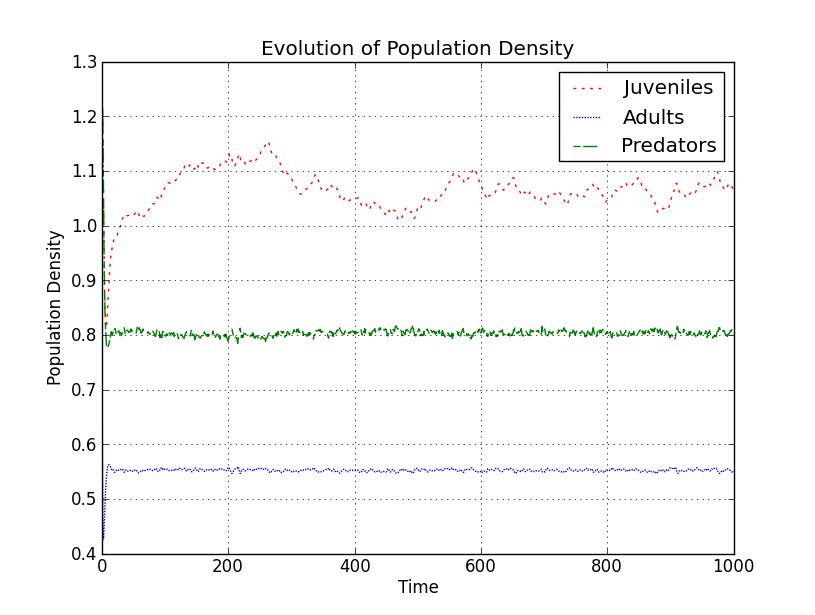
\includegraphics[width=\linewidth]{population_density_with_(white_noise)_ts.png}
  \caption{Juvenile, adult, and predator population densities over time with $\mu_P = 0.552$ and an independent noise term $\omega$ added to $\mu_P$ add each time step} 
\endminipage
\end{centering}
}
\end{figure}
\FloatBarrier

Looking at Fig. 33, it is clear that adding white-noise to the predator mortality rate close to the bifurcation point has little impact on the predator population density over time. This is fascinating in and of itself: the values that $\omega$ takes at many points pushes $\mu_P$ past the bifurcation point, yet the system does not  have an immediate and irreversible response. This may indicate that there are multiple time-scales occurring within the model. Though the addition of $\omega$ may not induce an immediate critical transition, it does have a clear impact on the stability of the  juvenile population density. Whereas we previously saw oscillatory behavior that would decay into a steady state, here we find constant fluctuations amongst all three population densities, with the largest fluctuations being seen clearly in the juvenile population density, $J$. This begs the question: have we eliminated the alternative stable state by adding a white noise term? To check, we must once more produce a time-series that has an increasing predator mortality rate, this time augmented by the white noise process. The following time-series begins with $\mu_P = 0.1$ and increases by $0.001+\omega$ for each "time-step" past $t=100$. 

\begin{figure}[!htb]
\centerline{
\begin{centering}
\minipage{\textwidth}
  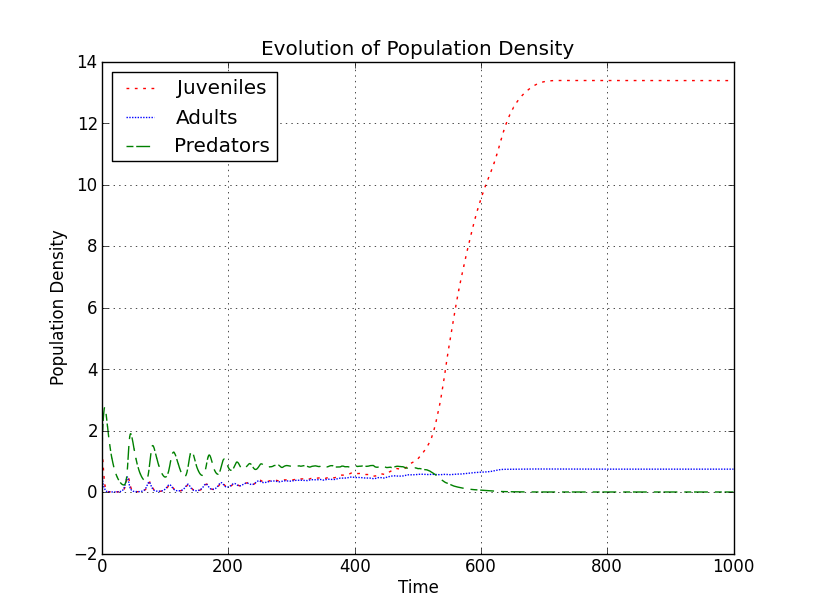
\includegraphics[width=\linewidth]{population_density_with_(white_noise)_ts_increasing.png}
  \caption{Juvenile, adult, and predator population densities with increasing $\mu_P$ and white noise} 
\endminipage
\end{centering}
}
\end{figure}
\FloatBarrier

We see two stable states in Fig. 34: one with predators ($P>0$) and one without ($P=0$). The alternative stable states therefore still exist, with the bifurcation occurring at $t\approx 5000$. Therefore, we may once more use our Early Warning Signals tool-kit to investigate. Unless worth a closer look, I will refrain from replicating the interior windows in larger figures as before. 

\begin{figure}[!htb]
\centerline{
\begin{centering}
\minipage{\textwidth}
  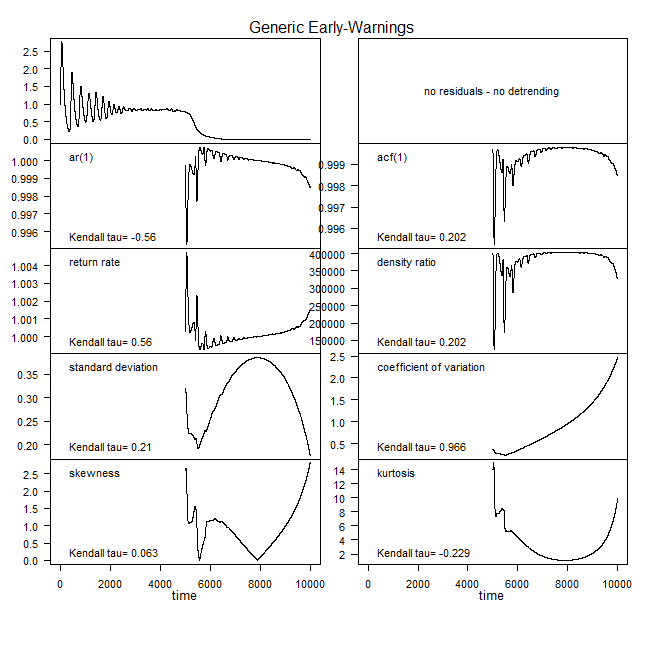
\includegraphics[width=\linewidth]{generic_ews_ts_pred_whitenoise.png}
  \caption{Output from "Early Warning Signals Tool-kit" in R for the predator population density ($P$) from our equation-based model with a white-noise process $\omega$ (\texttt{winsize = 50})} 
\endminipage
\end{centering}
}
\end{figure}
\FloatBarrier

As with the model specification without white noise, there are no conclusive early warning signals present in the predator population density time-series. We move on now to the early warning signals in the adult prey density. 

\begin{figure}[!htb]
\centerline{
\begin{centering}
\minipage{\textwidth}
  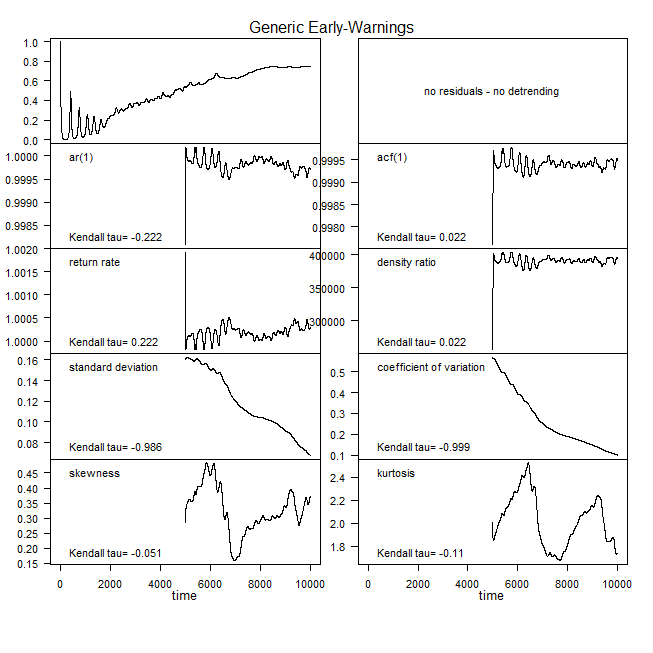
\includegraphics[width=\linewidth]{generic_ews_ts_adult_whitenoise.png}
  \caption{Output from "Early Warning Signals Tool-kit" in R for the adult population density ($A$) from our equation-based model with a white-noise process $\omega$ (\texttt{winsize = 50})} 
\endminipage
\end{centering}
}
\end{figure}
\FloatBarrier

Once more, Fig. 36 shows that there are no conclusive early warning signals present. It is worth noting that even though the measure of skewness may seem to show promise on visual inspection, the low Kendall tau value shows that there is little in the way of direct correlation between the two measurements. Finally, we will look at the early warning signals present in the juvenile prey population density.

\begin{figure}[!htb]
\centerline{
\begin{centering}
\minipage{\textwidth}
  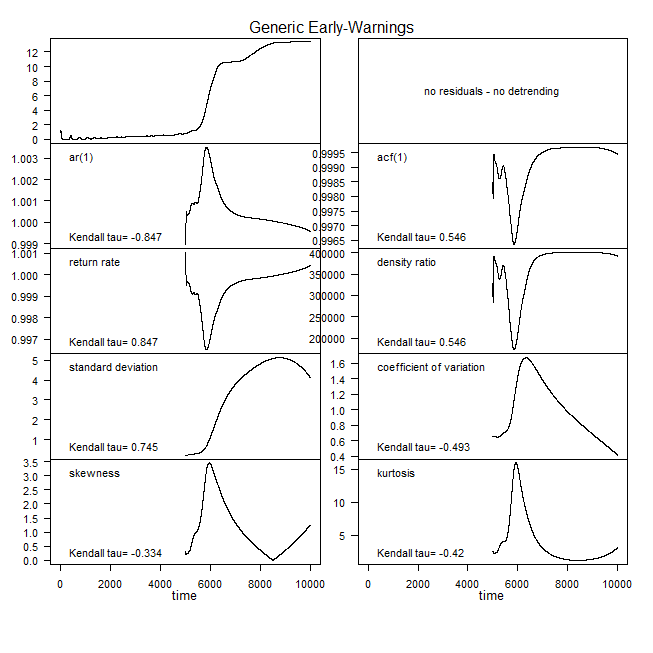
\includegraphics[width=\linewidth]{generic_ews_ts_juv_whitenoise.png}
  \caption{Output from "Early Warning Signals Tool-kit" in R for the juvenile population density ($J$) from our equation-based model with a white-noise process $\omega$ (\texttt{winsize = 50})} 
\endminipage
\end{centering}
}
\end{figure}
\FloatBarrier

Figure 37 offers some tantalizing evidence of a critical transition: the plot of ar(1) alone seems to point in the correct direction. However, the visualizations can be misleading. This can be seen very clearly if we separate the time-series data and the ar(1) visualization out and mark the point at which the critical transition occurs ($\mu_P \approx 0.553$): 

\begin{figure}[!htb]
\begin{centering}
\minipage{0.5\textwidth}
  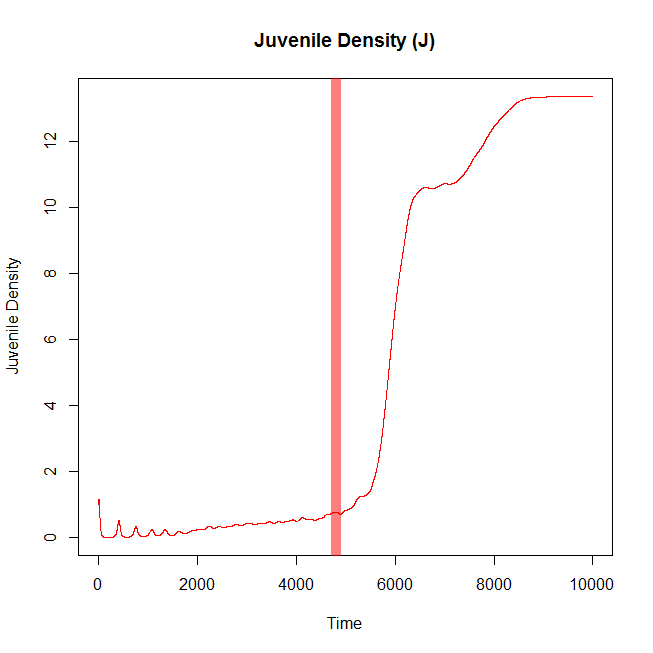
\includegraphics[width=\linewidth]{generic_ews_juv_whitenoise_ts.png}
  \caption{Time Series of $J$} 
\endminipage\hfill
\minipage{0.5\textwidth}
  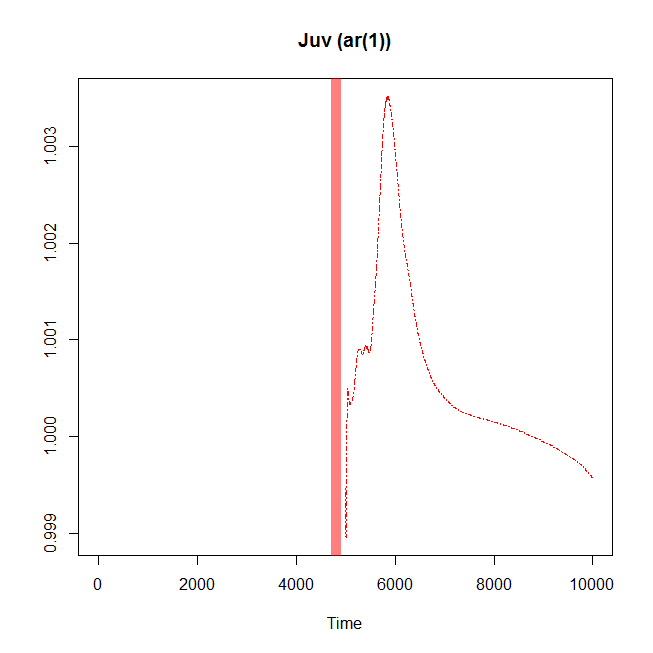
\includegraphics[width=\linewidth]{generic_ews_juv_whitenoise_ts_ar1.png}
  \caption{ar(1) $J$}
\endminipage\hfill
\end{centering}
\end{figure}
\FloatBarrier

This is easily explained. The model is first stochastically forced across the bifurcation point at time $t$ where $t=4822$. It never again goes below $\mu_P \approx 0.553$ after $t=4900$.\\

The close reader may have a nagging question on their mind at this point: what if the bifurcation takes place early in the time-series? The rolling window size of our ar(1) estimation function is 50\%. Therefore, the Early Warning Signals Tool-kit may be failing to find the bifurcation point because it has occurred \emph{before} the search function could find it. To see if shortening this window will be of use, we will shorten the size of our rolling window to 10\% so as to allow more of the time-series data to be incorporated into the search function.

\begin{figure}[!htb]
\centerline{
\begin{centering}
\minipage{\textwidth}
  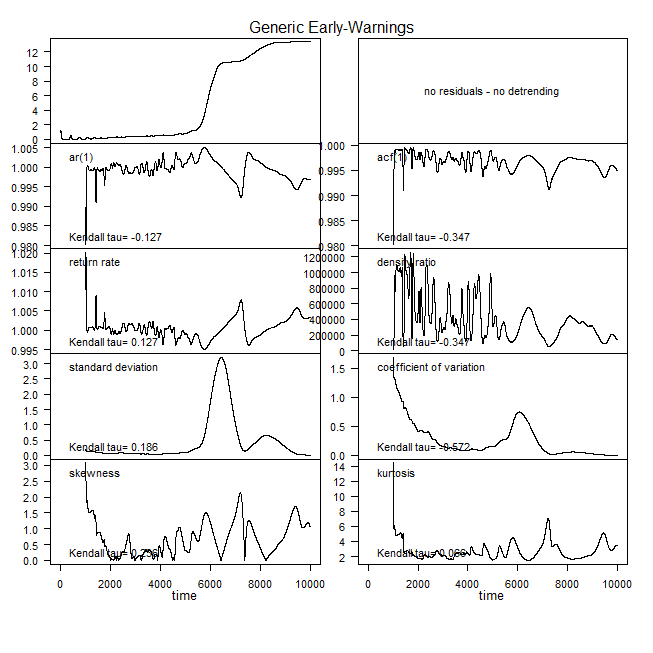
\includegraphics[width=\linewidth]{generic_ews_ts_juv_whitenoise_smallwindow.png}
  \caption{Output from "Early Warning Signals Tool-kit" in R for the juvenile population density ($J$) from our equation-based model with a white-noise process $\omega$ (\texttt{winsize = 10})} 
\endminipage
\end{centering}
}
\end{figure}
\FloatBarrier

Here, we see that the previously clear trend becomes far more ambiguous. It is an open question in time-series analysis as to how optimally specify the size of the rolling window. I acknowledge this open area of research as being vital to the extension of the theory surrounding critical transitions. Taking this into account, I have chosen to stick to a rolling window of 50\% of the time-series data to best approximate real-world situations \cite{Scheffer2001}. Additionally, I am utilizing a sliding (overlapping) window based on the idea that indicators should be estimated as data are becoming available. This is in contrast to the stance that model calibration (i.e., choosing a window-size that provides the desired result) is an effective method of inquiry. It is worth noting that a valid extension of this project would be to run an exhaustive analysis of early warning signals detection at all moving window values.\\

Moving forward, perhaps the addition of autocorrelated, or \emph{pink}, noise term will make the generic early warning signals more clear. The addition of autocorrelated environmental noise processes to ecological models has a long history in the literature \cite{Vasseur2014}\cite{Halley1996}\cite{Ghosh2012}\cite{Cohen1998}\cite{Ruokolainen2009}. In general terms, the addition of correlated noise to the model is meant to simulate environmental shocks that are temporally related--the the environmental stress of today may be related to the stresses of the environment found tomorrow.

%-------------------------------------------------
% Early warning signals in the equation-based model with pink noise
%-------------------------------------------------
\subsection{The ODE Model with Correlated (Pink) Noise}


We again will reference our equation-based model:
\begin{align}
	& \dfrac{dJ}{dt} = bA - \dfrac{J}{(1+J^2)} - \mu_JJ\\
	& \dfrac{dA}{dt} = \dfrac{J}{(1+J^2)} - APc - \mu_AA\\
	& \dfrac{dP}{dt} = P(cA - \mu_p)
\end{align}
However, we will now add a pink-noise term, $\zeta$, to the predator mortality rate. This term is a pink noise process with a power spectral density of $S(f) \propto \dfrac{1}{f^{\alpha}}$ where $0<\alpha<2$. This noise was synthesized through the use of a Fast Fourier Transform process.  Thus, the value of $\zeta$ at any point is statistically autocorrelated over time. Our new model becomes:

\begin{align}
	& \dfrac{dJ}{dt} = bA - \dfrac{J}{(1+J^2)} - \mu_JJ\\
	& \dfrac{dA}{dt} = \dfrac{J}{(1+J^2)} - APc - \mu_AA\\
	& \dfrac{dP}{dt} = P(cA - (\mu_p+\zeta))
\end{align}

I again choose to perturb only the predator mortality rate as this is the driving state variable which will force the model through the critical transition. These perturbations are not explicitly additive. If we set predator mortality quite close to the bifurcation point ($\mu_P = 0.552$) and perturb it by $\zeta$ at each time interval, we achieve an interesting result:

\begin{figure}[!htb]
\centerline{
\begin{centering}
\minipage{\textwidth}
  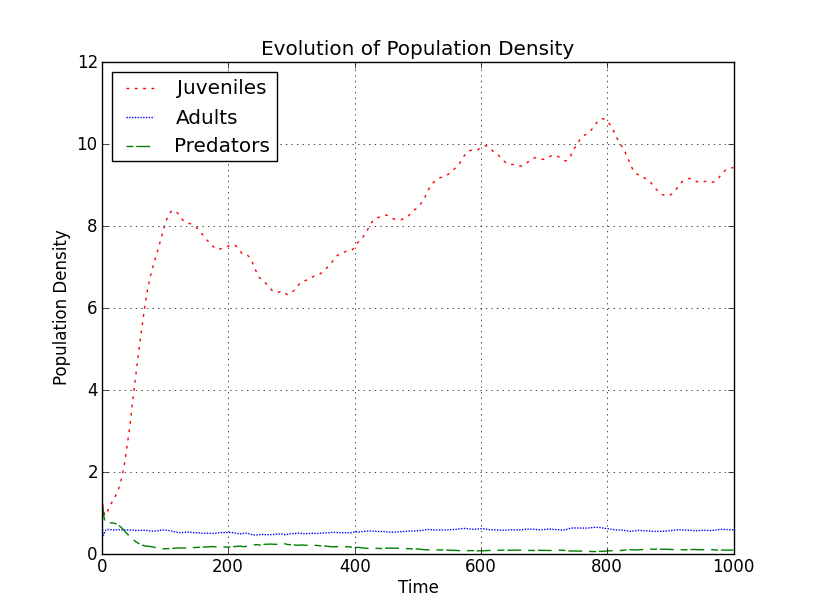
\includegraphics[width=\linewidth]{population_density_with_pink_noise.png}
  \caption{Juvenile, adult, and predator population densities over time with $\mu_P = 0.552$ and an autocorrelated noise term $\zeta$ added to $\mu_P$ add each time step} 
\endminipage
\end{centering}
}
\end{figure}
\FloatBarrier

Much as with the white-noise process, Fig. 41 makes clear that the addition of autocorrelated noise to the model has powerful impacts on the population densities of all three groups at a steady predator mortality rate. This is most likely caused by the autocorrelated nature of the noise term, $\zeta$--since each successive value is positively correlated to the value preceding it, positive trends are equally as likely to continue as negative trends, leading one to expect to see perturbation which push the model past the bifurcation point (and back over it again) rather quickly. To check that alternative stable states still exist, we must once more produce a time-series that has an increasing predator mortality rate, this time augmented by our pink noise process $\zeta$. The following time-series begins with $\mu_P = 0.1$ and increases by $0.001+\omega$ for each time-step past $t=100$. 

\begin{figure}[!htb]
\centerline{
\begin{centering}
\minipage{\textwidth}
  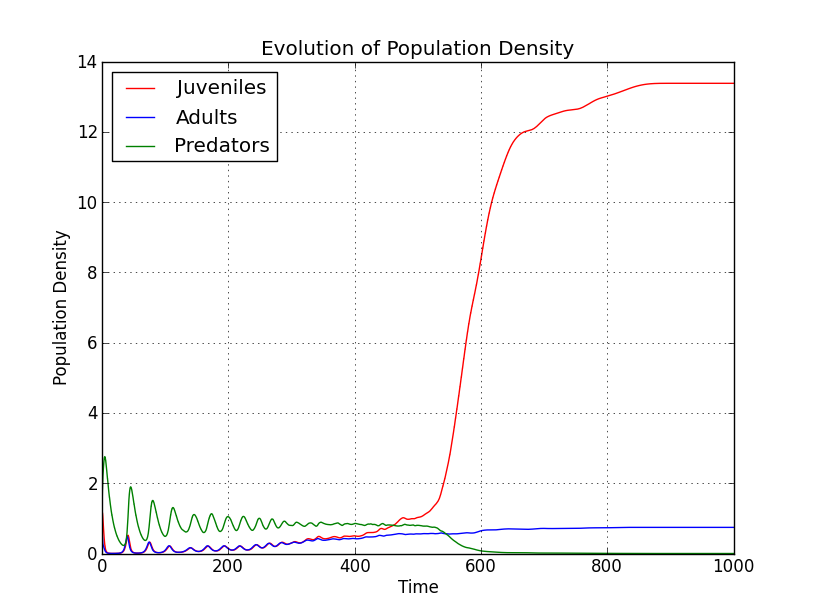
\includegraphics[width=\linewidth]{population_density_with_pink_noise_increasing.png}
  \caption{Juvenile, adult, and predator population densities with increasing $\mu_P$ and pink noise} 
\endminipage
\end{centering}
}
\end{figure}
\FloatBarrier

The alternative stable state with $P=0$ still exists. Therefore, we may once more use our Early Warning Signals tool-kit to investigate. Let us again examine the output files for the predator, adult, and juvenile population densities. 

\begin{figure}[!htb]
\centerline{
\begin{centering}
\minipage{\textwidth}
  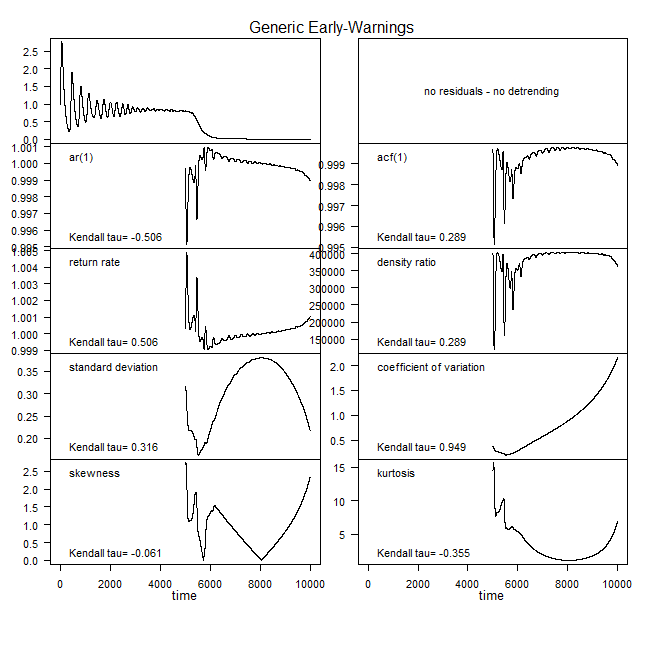
\includegraphics[width=\linewidth]{generic_ews_pred_pink_noise.png}
  \caption{Output from "Early Warning Signals Tool-kit" in R for the predator population density ($P$) from our equation-based model with a pink-noise process $\zeta$ (\texttt{winsize = 50}).} 
\endminipage
\end{centering}
}
\end{figure}
\FloatBarrier

\begin{figure}[!htb]
\centerline{
\begin{centering}
\minipage{\textwidth}
  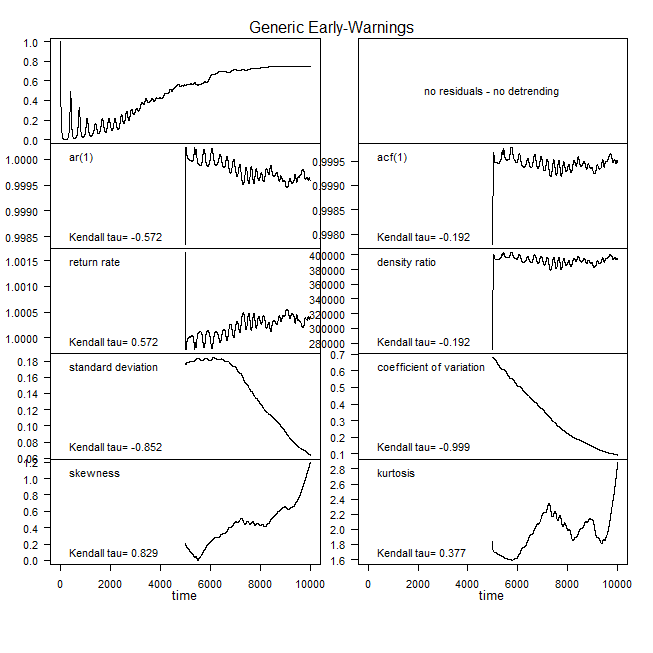
\includegraphics[width=\linewidth]{generic_ews_adult_pink_noise.png}
  \caption{Output from "Early Warning Signals Tool-kit" in R for the adult population density ($A$) from our equation-based model with a pink-noise process $\zeta$ (\texttt{winsize = 50}).} 
\endminipage
\end{centering}
}
\end{figure}
\FloatBarrier

\begin{figure}[!htb]
\centerline{
\begin{centering}
\minipage{\textwidth}
  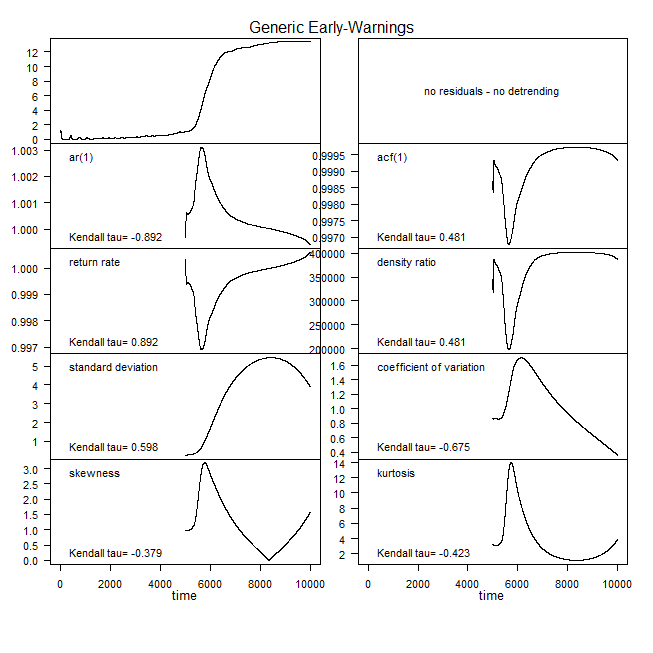
\includegraphics[width=\linewidth]{generic_ews_juv_pink_noise.png}
  \caption{Output from "Early Warning Signals Tool-kit" in R for the juvenile population density ($J$) from our equation-based model with a pink-noise process $\zeta$ (\texttt{winsize = 50}).} 
\endminipage
\end{centering}
}
\end{figure}
\FloatBarrier

Fig. 43, 44, and 45 tell the same story we've previously seen--the early warning signals for this particular modeling specification are absent before the critical transition even when either independent (white) or correlated (pink) noise processes are added to the equations \footnote{We note that the ar(1) for our juvenile population density is moving in the correct direction. This is a finding explained in \cite{Boerlijst2013}: the state variable of interest, predator density ($P$) shows no early warning signals, yet the juvenile density ($J$) sometimes does. In a real-world situation, this may mean ecosystem-wide monitoring regimes may be useful in understanding population variations under pressure}.  Though this certainly does not wholly disprove the theory that systems with alternative stable states exhibit early warning signals in a universal sense, it is an empirical example of such a situation where the ability to presage a collapse may be impossible.\\

Or is it? Though we have tested this situation in a differential equation model, we have not considered other modeling paradigms. There is the potential that modeling this same system in an agent-based environment may yet yield the early warning signs for critical transitions that we aim to discover, especially if one believes that critical transitions can themselves be emergent phenomena. If, for example, we hope to protect an ecologically or environmentally important species under the threat of extinction, it is imperative that we know if certain model specifications may exhibit such emergent behaviors that other models may miss. With that in mind, let us explore an agent-based model of the predator-prey system of ODEs.


%-------------------------------------------------
%-------------------------------------------------
%-------------------------------------------------
%-------------------------------------------------
% SECTION THREE
%-------------------------------------------------
%-------------------------------------------------
%-------------------------------------------------
%-------------------------------------------------
%-------------------------------------------------
\section{The Agent-Based Model}

%-------------------------------------------------
% Building the agent-based model
%-------------------------------------------------
\subsection{Constructing the Agent-Based Model}

My agent-based model \footnote{The ABM code is reprinted in full in the supplemental information} was constructed in the Python programming language and built upon the framework provided by the \texttt{PyCX} package. The spatial environment we are modeling may be either a torus (i.e., the agents may wrap-around from one end of the modeling area to the other) or a bounded square (i.e., the agents can "hit the wall" and are enclosed). Agents are initially placed into the environment at random. Each agent may be one of three classes: juvenile prey, adult prey, or predator. All individuals may move freely about the environment and move according to the same rules (a random walk). The rules governing the behavior of each agent are based upon the terms in our ODE model. They are:
\begin{itemize}
	\item Juvenile prey may (1) become adult prey or (2) die. 
	\item Adult prey may (1) give birth to juvenile prey, (2) be consumed by a predator, or (3) die. 
	\item Predators may (1) consume adult prey, (2) give birth to new predators, or (3) die. 
\end{itemize}
These behaviors are modeled as probabilistic rule-functions that each agent completes during a time step. All agents update simultaneously. Though not strictly necessary, I found it useful to create a graphic-user interface (also known as a GUI) to visualize what was occurring within the model space. The GUI is shown in Fig. 46.

\begin{figure}[!htb]
\centerline{
\begin{centering}
\minipage{\textwidth}
  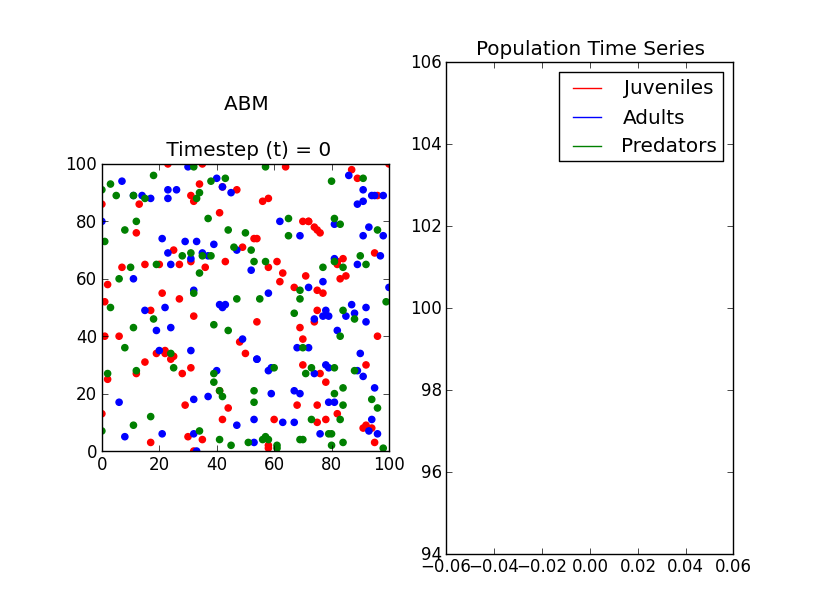
\includegraphics[width=\linewidth]{abm_noncalibrated_setup.png}
  \caption{ABM Model at $t=0$. Juvenile agents are represented by red dots, adults by blue dots, and predators by green dots.} 
\endminipage
\end{centering}
}
\end{figure}
\FloatBarrier

Figure 47 shows the GUI after it has run for several time-steps.

\begin{figure}[!htb]
\centerline{
\begin{centering}
\minipage{\textwidth}
  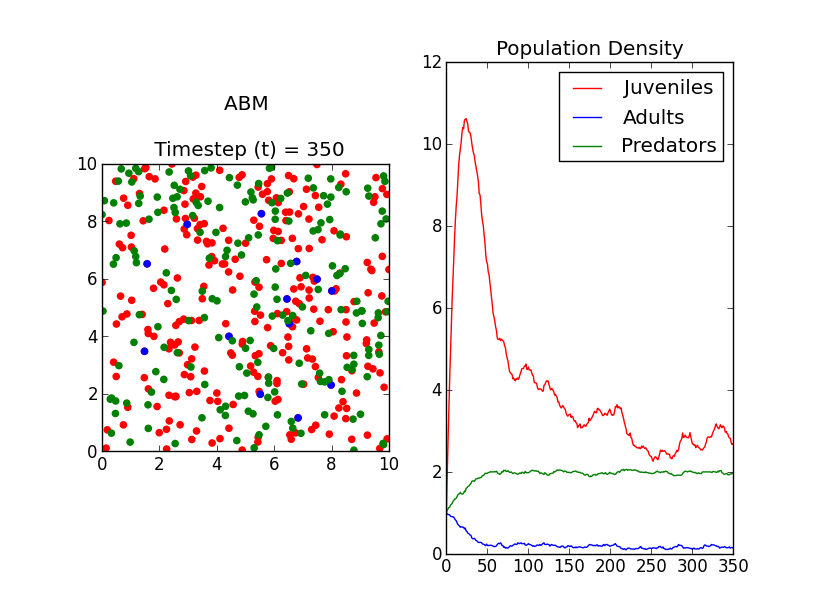
\includegraphics[width=\linewidth]{abm_noncalibrated_350steps.png}
  \caption{ABM Model at $t=350$.} 
\endminipage
\end{centering}
}
\end{figure}
\FloatBarrier

The ABM outputs the time-series information as a .csv file to be used for later statistical analysis. Now that I've constructed the ABM, we must calibrate its various parameters to the ODE model specifications to make sure that we are comparing "apples to apples".

%-------------------------------------------------
% Calibrating the agent-based model
%-------------------------------------------------
\subsection{Calibrating the Agent-Based Model}

There are several issues that we must work through before we can compare the ABM to the ODE model. These issues include the difference between population densities and total population counts, the conversion of non-spatially reliant rules for behavior to those that are spatially-explicit, and the calibration of time-scales across the two models. I show my reasoning below.

\subsubsection{Density v. Individuals}

The ODE model is express in terms of population densities, not the total population. I will address this issue in two ways. First,  I have consistently utilized an equal density ratio as the "starting point" in all of my model implementations (i.e., we've always set $P$,$A$, and $J$ equal to 1 while numerically solving our ODEs). If I maintain the same ratios in my ABM implementations (by initializing the model with the same number of predators, adults, and juveniles) and set the total size of the modeling environment (length and width) equal to this value, I will achieve equivalent initial population densities. In all following model implementations, I have chosen to begin with 100 individuals of each agent class. The length and width of the modeling environment has been set to ten. Though the unit-less nature of this value may give pause to some, it is best to think of this value as a measurement of "on-screen centimeters". Therefore, when we divide the initial agent populations (100) by the area of the environment (100) we achieve an initial population density of 1. Additionally, when recording the time-series output, I have divided the total number of agents in each class by the area of the modeling environment. Therefore, the time-series output of the ABM model is qualitatively and quantitatively the same as that of my ODE model.

\subsubsection{Spatial v. Non-spatial Rules}

For reference, let's take one more glance at the ODE model: 
\begin{align}
	& \dfrac{dJ}{dt} = bA - \dfrac{J}{(1+J^2)} - \mu_JJ\\
	& \dfrac{dA}{dt} = \dfrac{J}{(1+J^2)} - APc - \mu_AA\\
	& \dfrac{dP}{dt} = APc - \mu_pP
\end{align}
Now let's examine how each of these terms becomes incorporated into the ABM. \\

The term $bA$ can be thought of as the fecundity term. In the ODE, it shows the addition to the juvenile population density which comes from the reproduction by adults. It is not spatially-explicit: reproduction occurs whether or not individual adults are within proximity to one another. For the ease of comparison, I have maintained this distinction in the ABM model. Adults breed according to a probabilistic rule: at each-time step, a random number between 0 and 1 is generated, and if this number is less than the adult-reproduction rate ($b$), the adult successfully breeds and creates a new juvenile. As in the ODE model, I have set $b=1$, thus all adults breed at each-time step. \\

The term $ \dfrac{J}{(1+J^2)}$ is the non-linear maturation rate of the juveniles into adulthood. It is also not spatially-explicit. I have maintained this in the ABM. The juvenile maturation rate updates at each call of the \texttt{step()} function according to the following equation:
\begin{align*}
	& \text{Juvenile Maturation Rate}\,=\dfrac{\dfrac{\text{Number of Juvneiles}}{A}}{\left(1+\left(\dfrac{\text{Number of Juveniles}}{A}\right)^2\right)}
\end{align*}
where $A$ is the total area of the environment size. This makes sure that our maturation rates are equivalent across models.\\

Our mortality terms, $\mu_P$, $\mu_A$, and $\mu_J$ are not spatially-explicit. They will, however, pose a problem to be addressed below.\\

Our final term, $APc$, is spatially-explicit within our ABM. As we are dealing with the behavior of individuals as opposed to the system as a whole, I will model individual interactions in order to accurately model predation. In the model, the predator agents only consume adult prey agents if they come within a certain distance (here modeled as approximately 0.01\% of the total area of the environment, or $\left(\dfrac{1}{1000}(100)\right)^2=0.01$ \footnote{The addition of this "detection distance" to the model adds in another possible variable by which to force the model through a bifurcation. However, it is unlikely that detection abilities are subject to stochastic forcing in most realistic ecological settings. I will therefore ignore this topic as being outside the scope of this investigation, but note that it may prove a ripe area of investigation.}. This term also controls the reproduction rate of our predators. As in the ODE model, we use a value of $c=1$. Therefore, for the sake of model simplicity every time a predator consumes an adult prey that predator successively breeds. 

%-------------------------------------------------
% Time scales across the models
%-------------------------------------------------
\subsubsection{Time Scales Across the Models}

I will now return to the problems of our mortality rates as mentioned above. As I had mentioned in discussion about Fig. 49, it seems that there may be multiple time-scales taking place within the ODE model, most likely driven by the differences in the mortality rates between our model components (the predator, adults, and juveniles). This causes a problem for us as we try to calibrate our ABM to the ODE model: for example, how can we know that the mortality rate for the adult population density in the ODE model ($\mu_A = 0.1$) is equivalent to the same mortality rate for our ABM? \\

First, we must check and see how long it takes each individual component of the ODE model to go extinct: i.e., if we set the other two population densities to zero, how many iteration will it take for the remaining population to reach zero as well? Note that in order to perform this analysis, I've had to suppress some terms. For the adults, I've had to suppress the fecundity term ($bA$) as this would give rise to a juvenile population and a steady-state equilibrium would be reached. For the juveniles, I've had to suppress the maturation rate term $\left(\dfrac{J}{(1+J^2)}\right)$ or the same problem would arise. 

\begin{center}
	\begin{tabular}{| l | l | }
	\hline
	Variable & $t$ of Extinction for $\mu = 0.1$ (ODE) \\ \hline
	$P$  & $t = 100$ ($P = 0.0000449$)  \\ \hline
	$A$ & $t = 100$ ($A = 0.0000496$) \\ \hline
	$J$  & $t=10$ ($J = 0.0000767$)  \\ \hline
	\end{tabular}
 \end{center}

It is worth noting that the \texttt{ODEINT} routine in Python will asymptotically approach zero but never quite reach it. I have therefore chosen to take the value at which the population density drops below $10^{-5}$ as being equivalent to zero. Now, let's set all the mortality rates to $\mu = 0.1$ for our ABM and perform the same test:

\begin{center}
	\begin{tabular}{| l | l | }
	\hline
	Variable & $t$ of Extinction for $\mu = 0.1$  (ABM) \\ \hline
	$P$  & $t \approx 50 (49.93)$\\ \hline
	$A$ & $t \approx 50 (49.69)$ \\ \hline
	$J$  & $t \approx 50 ( 49.22)$  \\ \hline
	\end{tabular}
 \end{center}

Here, we average the extinction time ($t$) for one hundred runs of the model and rounded up to the nearest integer. What we see is that there is a discrepancy between the ratio of extinction times between the ODE model and the ABM. In the ABM, we see that each agent class tends to go extinct at roughly the same time when given the same mortality rate. This is intuitively what we should have expected: since mortality is being modeled in each agent class in exactly the same way, their times to extinction should be equivalent. Let's examine both the ODE and the ABM from the mortality rates specified in \cite{Boerlijst2013} ($\mu_P = 0.1$, $\mu_A = 0.1$, $\mu_J = 0.05$). Note that we are using a value of $\mu_P = 0.1$ as a reference point even though we are going to be increasing this value incrementally up to a critical transition. 

\begin{center}
	\begin{tabular}{| l | c | l | }
	\hline
	Variable & $\mu$ & $t$ of Extinction (ODE) \\ \hline
	$P$  & $\mu_P = 0.1$ & $t = 100$ ($P = 0.0000449$)  \\ \hline
	$A$ & $ \mu_A = 0.1$ & $t = 100$ ($A = 0.0000496$) \\ \hline
	$J$  & $\mu_J = 0.05 $ & $t=11$ ($J = 0.0000443$)  \\ \hline
	\end{tabular}
 \end{center}

We see that there is relatively little change in the ratio of extinction times. The juvenile prey population density reaches the threshold one time-step later than previously, but the difference between the actual values is quite low. It's therefore safe to say that the distribution is approximately the same: juvenile population density, in the absence of any other interaction terms, seems to go to zero approximately ten times faster than the predators or adults. And in the ABM, we observe:

\begin{center}
	\begin{tabular}{| l | c | l | }
	\hline
	Variable & $\mu$ & $t$ of Extinction (ABM) \\ \hline
	$P$  & $\mu_P = 0.1$ &  $t \approx 50 (49.91)$\\ \hline
	$A$ & $\mu_A = 0.1$ & $t \approx 50 (49.79)$ \\ \hline
	$J$  & $\mu_J = 0.05 $ & $t \approx 100 ( 99.65)$  \\ \hline
	\end{tabular}
 \end{center}

We see that an incremental decrease of 0.05 in the mortality rate for the juveniles results in a doubling of the juvenile time to extinction. Therefore, to achieve the same rate of extinction as we see in the ODE model (where the juveniles die off at a rate that is ten-times faster than the predators and adults), we can simply add 0.5 ($10\times 0.05$) to $\mu_J = 0.1$:

\begin{center}
	\begin{tabular}{| l | c | l | }
	\hline
	Variable & $\mu$ & $t$ of Extinction (ABM) \\ \hline
	$P$  & $\mu_P = 0.1$ &  $t \approx 50 (49.95)$\\ \hline
	$A$ & $\mu_A = 0.1$ & $t \approx 50 (49.80)$ \\ \hline
	$J$  & $\mu_J = 0.6 $ & $t \approx 5 ( 4.97)$  \\ \hline
	\end{tabular}
 \end{center}

And, finally, to normalize between the ODE and the ABM, we can simply adjust the values for our mortality rates:

\begin{center}
	\begin{tabular}{| l | c | l | }
	\hline
	Variable & $\mu$ & $t$ of Extinction (ABM) \\ \hline
	$P$  & $\mu_P = 0.05$ &  $t \approx 100 (100.75)$\\ \hline
	$A$ & $\mu_A = 0.05$ & $t \approx 100 (99.340)$ \\ \hline
	$J$  & $\mu_J = 0.50 $ & $t \approx 10 ( 10.06)$  \\ \hline
	\end{tabular}
 \end{center}

Upon repeated iterations of the model, I observed that these mortality rates always lead to extinction events. However, if I scale the mortality rates down by $100\%$, I find that the model does not lead to arbitrary extinction events and we achieve population distribution remarkably similar to those we see in Fig 33. Therefore, the final mortality rates for our ABM are:

\begin{center}
	\begin{tabular}{| l | c | }
	\hline
	Variable & $\mu$   \\ \hline
	$P$  & $\mu_P = 0.005$ \\ \hline
	$A$ & $\mu_A = 0.005$  \\ \hline
	$J$  & $\mu_J = 0.05 $   \\ \hline
	\end{tabular}
 \end{center}

Which, when implemented, provides the output found in Fig. 48.

\begin{figure}[!htb]
\centerline{
\begin{centering}
\minipage{\textwidth}
  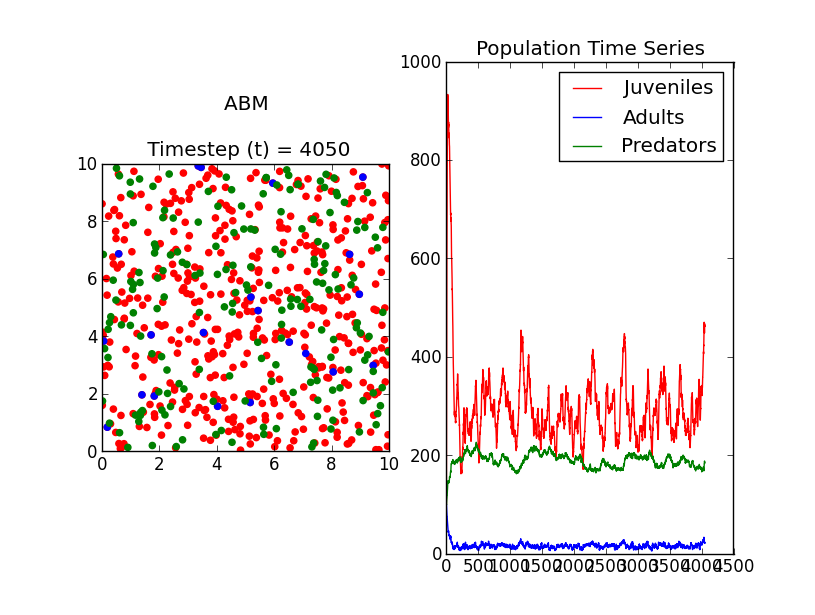
\includegraphics[width=\linewidth]{abm_calibrated_example.png}
  \caption{ABM Model at $t=4050$.} 
\endminipage
\end{centering}
}
\end{figure}
\FloatBarrier

Now that our models are calibrated, we can proceed with our analysis.


%-------------------------------------------------
%-------------------------------------------------
%-------------------------------------------------
%-------------------------------------------------
% SECTION FOUR
%-------------------------------------------------
%-------------------------------------------------
%-------------------------------------------------
%-------------------------------------------------
%-------------------------------------------------
\section{Results}

In this section I will analyze the output of the agent-based model under several conditions. I will look for early warning signals in the model under both "fast" and "slow" perturbation rates. I will do so under conditions of a linearly increasing mortality rate, an increasing mortality rate with Gaussian white noise, and an increasing mortality rate subject to autocorrelated pink noise. I will then discuss the findings and posit potential avenues for further investigation.


%-------------------------------------------------
% Toroidal v. Non-toroidal ABM
%-------------------------------------------------
\subsection{Toroidal v. Non-toroidal ABM}

The ability to exploit spatial interactions into a model is one of more powerful abilities of agent-based modeling. However, after many successive runs of our ABM, I have found that the shape of the environment has a relatively negligible impact on our results. The typical difference is best displayed in comparing Figures 49 and 50:

\begin{figure}[!htb]
\begin{centering}
\minipage{0.5\textwidth}
  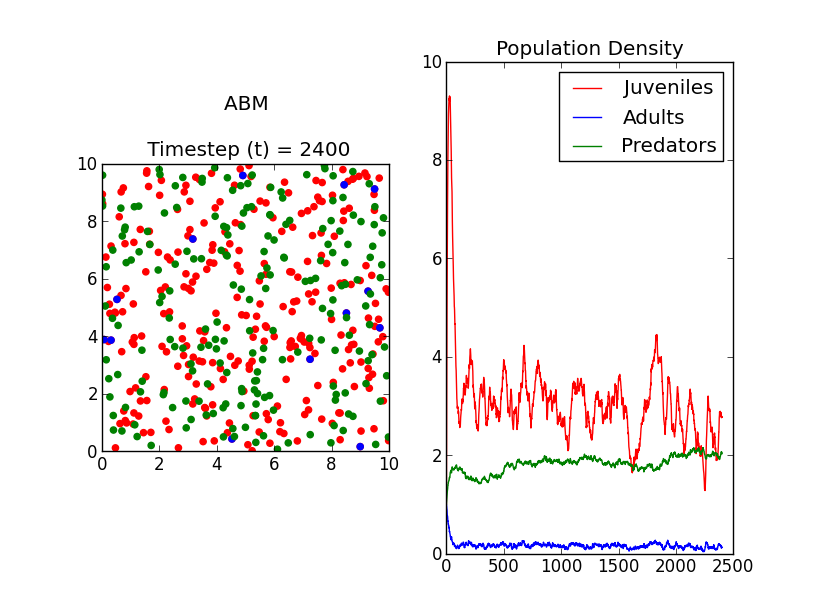
\includegraphics[width=\linewidth]{abm_with_torus.png}
  \caption{Time-series of ABM with toroidal boundary conditions} 
\endminipage\hfill
\minipage{0.5\textwidth}
  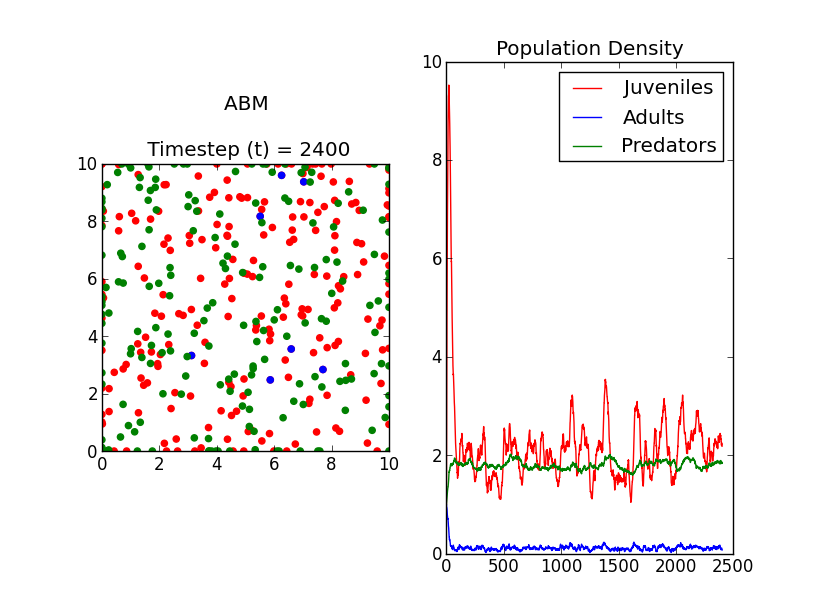
\includegraphics[width=\linewidth]{abm_no_torus.png}
  \caption{Time-series of ABM with non-toroidal boundary conditions}
\endminipage\hfill
\end{centering}
\end{figure}
\FloatBarrier

Figure 49 is the output of the ABM with toroidal ("wrap-around") environmental conditions enforced. Figure 50 is the output of the ABM with non-toroidal ("sandbox") environmental condition enforced. What we see is a relatively lower mean population density for the juvenile prey species in the non-toroidal environment. There are a variety of explanations, but my hypothesis is that the most likely reason for this discrepancy is that the encounter rate is slightly increased by the non-toroidal environment. The move function, a random-walk process, is the same between both environmental implementations. Agents that move against a border in the non-toroidal environment may therefore spend relatively more time in the same spot than those in a non-toroidal environment. Such agents may therefore have a subsequently increased risk of predation. I find that over the variety of implementations of the model (including fast and slow perturbation and various types of noise), the environmental shape has no statistical relevance to our question of study. Questions of environmental shape will thus be disregarded in further analysis.

%-------------------------------------------------
% Fast vs. Slow Perturbations
%-------------------------------------------------
\subsection{Fast v. Slow Perturbations}

In our hunt for clear early warning signals, it's important that we examine the rate of temporal disturbances to the model and their potential influences on EWS detection. As I mentioned in Section 1, critical transitions may only be discoverable if the perturbation to the system is fast \emph{relative} to the global temporal scale of the model. Thus, I will examine if there are differences that occur with perturbations at different periods. To model this, we have disturbed the predator mortality rate in several ways. With an initial predator mortality of 0.005, we first begin adding 0.0001 to this value every fifty time-steps. We call this perturbation "slow" relative to the temporal scale of the model. Fig. 51 displays the final output from this model.

\begin{figure}[!htb]
\centerline{
\begin{centering}
\minipage{\textwidth}
  \includegraphics[width=\linewidth]{abm_slow_shock.png}
  \caption{ABM model with predator mortality rate increasing by 0.0001 every 50 time-steps.} 
\endminipage
\end{centering}
}
\end{figure}
\FloatBarrier

We do not visually see the discontinuous shift between stable states that typifies a critical transition. If we have set the perturbations to a timescale that is "too slow", we may allow the system to react in a linear (and gradual) way to the systemic shock. Will our Early Warning Signals Tool-kit, however, find a critical transition in the time-series data?

\begin{figure}[!htb]
\centerline{
\begin{centering}
\minipage{\textwidth}
  \includegraphics[width=\linewidth]{abm_slowshock_ews.png}
  \caption{Output from "Early Warning Signals Tool-kit" in R for the predator population density ($P$) from the ABM with predator mortality increasing by 0.0001 every 50 time steps. (\texttt{winsize = 50})} 
\endminipage
\end{centering}
}
\end{figure}
\FloatBarrier

We do not see the desired trends in our measures of ar(1), standard deviation, coefficient of variation, kurtosis, skewness, or the density ratio. The "slow" shocks to the system did not create a critical transition in the ABM. \\

Next, I will model a "fast" perturbation to the system. With an initial predator mortality of 0.005, we begin adding 0.0001 to this value \emph{every} time-step.  Fig. 53 displays the final output from this model.

\begin{figure}[!htb]
\centerline{
\begin{centering}
\minipage{\textwidth}
  \includegraphics[width=\linewidth]{abm_fast_shock.png}
  \caption{ABM model with predator mortality rate increasing by 0.0001 every time-step.(Note: The predator population density ($P$) reached zero on the final time-step, even though the plot is not visually representative of this event.)} 
\endminipage
\end{centering}
}
\end{figure}
\FloatBarrier

We once again do not have visual confirmation of a discontinuous shift between stable states in the predator population density ($P$). We note, however, that one may notice a rapid increase in the juvenile population densities after $t \approx 150$. We are curious, however, about the ability to detect early warning signals in the population undergoing the critical transition. Our Early Warning Signals Tool-kit output in Figure 54 is equally ambiguous.

\begin{figure}[!htb]
\centerline{
\begin{centering}
\minipage{\textwidth}
  \includegraphics[width=\linewidth]{abm_fastshock_ews.png}
  \caption{Output from "Early Warning Signals Tool-kit" in R for the predator population density ($P$) from the ABM with predator mortality increasing by 0.0001 every time step. (\texttt{winsize = 50})} 
\endminipage
\end{centering}
}
\end{figure}
\FloatBarrier

We note here that the standard deviation and coefficient of variation show promise as potential EWS, along with kurtosis. There are complications to our current modeling implementation, however, that may prevent us from utilizing these as a robust EWS. The predator mortality rate is being perturbed every time-step from the moment of model initialization. We therefore may not have allowed the model enough time to move past initial transitory behavior and achieve model stability (a process known as "burning-in" in the agent-based modeling literature). What if we once again model "fast" perturbations, but only begin to increase the predator mortality after 1000 time-steps? Figure 55 displays the results.

\begin{figure}[!htb]
\centerline{
\begin{centering}
\minipage{\textwidth}
  \includegraphics[width=\linewidth]{abm_fast_shock_burnin.png}
  \caption{ABM model with predator mortality rate increasing by 0.0001 every time-step after time-step 1000.} 
\endminipage
\end{centering}
}
\end{figure}
\FloatBarrier

Our subsequent analysis of the EWS are shown in Fig. 56
\begin{figure}[!htb]
\centerline{
\begin{centering}
\minipage{\textwidth}
  \includegraphics[width=\linewidth]{abm_fastshock_burnin_ews.png}
  \caption{Output from "Early Warning Signals Tool-kit" in R for the predator population density ($P$) from the ABM with predator mortality increasing by 0.0001 every time step after time-step 1000. (\texttt{winsize = 50})} 
\endminipage
\end{centering}
}
\end{figure}
\FloatBarrier

This is promising! In fact, we here observe many similarities between Figure 56 and Figure 10: increasing ar(1), increasing standard deviation, an increasing density ratio, and an increasing coefficient of variation. This is particularly important to potential applications because unlike the ODE model, we are here finding potential early warning signals in the species being disturbed. This is a qualitatively different outcome than what was found in \cite{Boerlijst2013}. This could have a myriad of useful applications, especially in the management of ecosystems under stress: the ability to model community interactions in such a way as to see early warning signals in the monitored species of interest would be of exceptional value. But before we discuss these findings further, let's continue with our analysis and introduce an independent noise process to the predator mortality rate.

%-------------------------------------------------
% Perturbations with White Noise
%-------------------------------------------------
\subsection{Perturbation with White Noise}

First, let's examine what the addition of an independent, Gaussian white noise term (with $\mu=0$ and $\sigma = 0.005$) does to the behavior of the system. The results of this are found in Fig. 57. 

\begin{figure}[!htb]
\centerline{
\begin{centering}
\minipage{\textwidth}
  \includegraphics[width=\linewidth]{abm_whitenoise.png}
  \caption{ABM model with predator mortality rate being perturbed every time-step by the white noise term $\omega$ ($\mu=0$ and $\sigma = 0.005$).} 
\endminipage
\end{centering}
}
\end{figure}
\FloatBarrier

We note that the addition of the Gaussian white noise does not drastically alter the system behavior. Unlike the ODE model, we already have a stochastic element operating in the ABM (via the various function controlling movement and mortality) and therefore did not expect to see drastic changes to the system behavior. Following the same burn-in procedure as before, I will now show the behavior of the model after an increase the predator mortality rate by ($0.0001 + \omega $) after time-step 1000: 

\begin{figure}[!htb]
\centerline{
\begin{centering}
\minipage{\textwidth}
  \includegraphics[width=\linewidth]{abm_fast_shock_whitenoise.png}
  \caption{ABM model with predator mortality rate being perturbed every time-step by an additive noise function (0.0001 + $\omega$) after time-step 1000.} 
\endminipage
\end{centering}
}
\end{figure}
\FloatBarrier

I once again note that in Fig. 58, the predator population density ($P$) reaches zero at $t\approx 1300$. Are there EWS present in this data? 

\begin{figure}[!htb]
\centerline{
\begin{centering}
\minipage{\textwidth}
  \includegraphics[width=\linewidth]{abm_whitenoise_ews.png}
  \caption{Output from "Early Warning Signals Tool-kit" in R for the predator population density ($P$) from the ABM with predator mortality increasing by (0.0001 + $\omega$) every time step after time-step 1000. (\texttt{winsize = 50})} 
\endminipage
\end{centering}
}
\end{figure}
\FloatBarrier

This particular output from the Early Warning Signals Tool-kit suffers the same problems as in our ODE model: certain signals are present (such as the positively-trending ar(1) and spectral density ratio values), but they only display the theorized behavior \emph{after} the population has collapsed. Critically, it seems that the addition of a white-noise process to our ABM may in fact dampen the statistical oscillations which are providing the early warning signals. This can be problematic, as the addition of various types of noise processes have a wide history in the ecological literature and may have useful modeling properties. We note, however, that further investigation of the addition of white noise terms to the model (such as varying the white noise fluctuation temporally, or applying them across all the mortality rates) may be useful. \\

As with our ODE model, let us now turn to examining the addition of an autocorrelated $\left(\dfrac{1}{f}\right)$ noise function to the predator mortality rate.


%-------------------------------------------------
% Perturbations with Pink Noise
%-------------------------------------------------
\subsection{Perturbation with Pink Noise}

We first examine what the addition of a autocorrelated pink noise term ($\zeta$) does to the behavior of the system. The results of this are found in Fig. 60. 

\begin{figure}[!htb]
\centerline{
\begin{centering}
\minipage{\textwidth}
  \includegraphics[width=\linewidth]{abm_pinknoise.png}
  \caption{ABM model with predator mortality rate being perturbed every time-step by the pink noise term $\zeta$.} 
\endminipage
\end{centering}
}
\end{figure}
\FloatBarrier

Much as with the addition of the independent white noise term, we did not expect (nor do we find) drastic differences in our model output across multiple iterations of the ABM with an autocorrelated noise perturbation. Fig. 61 will examine the EWS. 

\begin{figure}[!htb]
\centerline{
\begin{centering}
\minipage{\textwidth}
  \includegraphics[width=\linewidth]{abm_pinknoise_ews.png}
  \caption{Output from "Early Warning Signals Tool-kit" in R for the predator population density ($P$) from the ABM with predator mortality increasing by (0.0001 + $\zeta$) every time step after time-step 1000. (\texttt{winsize = 50})} 
\endminipage
\end{centering}
}
\end{figure}
\FloatBarrier

Oncen again, the EWS present are ambiguous. We see partial positive EWS in the values of ar(1) and the density ratio, but both show counterintuitive behavior near the transition point. The ar(1) values plateau as we approach the proposed bifurcation point, whereas the density ratio promptly reverses its trend. 


%-------------------------------------------------
%-------------------------------------------------
%-------------------------------------------------
%-------------------------------------------------
% DISCUSSION
%-------------------------------------------------
%-------------------------------------------------
%-------------------------------------------------
%-------------------------------------------------

\section{Discussion}

Throughout the course of this investigation, I have come to several conclusions regarding the nature of critical transitions in agent-based modeling and their level of detectability. Here, I will return to each and address them more fully.

\begin{itemize}
	\item \emph{The addition of independent or autocorrelated noise processes to a model system with a known bifurcation does not necessarily provide any additional ability to detect early warning signals for critical transitions in that model}.
\end{itemize}

As we discovered in Sections 2.7 and 2.8, the addition of varying types of stochastic fluctuations to the ODE model did not enhance the ability to detect early warning signals for critical transitions in the system. Though I had previously hypothesized that the fluctuations these stochastic shocks would impart on the system may help to amplify the background statistical variations in such a way as to assist in the discovery of EWS, this particular model example has shown my intuition incorrect. There are further extensions and implementations of this model which may yet prove useful for analysis. For example, applying similar and dissimilar noise processes to all of the mortality rates simultaneously may more accurately reflect stochastic environmental forcing in real-world environments. However, it is worth noting that the addition of noise terms to our models did not assist in the discovery of critical transitions in either the ODE or ABM model specifications. \\

\begin{itemize}
	\item \emph{It may be possible to create agent-based models which are calibrated to the specifications of an ODE model and to achieve qualitatively similar behavior between the two.}
\end{itemize}

One of the more innovative areas of research in this project was the calibration of an ABM to an ODE model so as to conduct comparative analysis of their results. I believe that the process of translating model specifications across modeling paradigms is instructive in a variety of ways: the act of calibrating an ABM involves searching for a deeper understanding of temporal scale, transitory behavior, and equilibrium states of the ODE model. Besides being of strictly academic interest, I believe such analyses may prove useful in a variety of real-world policy applications.\\

As I discussed in the introduction to this project, agent-based models are quite useful when seeking to understand emergent phenomena of a system: that is, systemic behavior that arises from the aggregated behavior of individuals and is not present in the individuals themselves. I had hypothesized that critical transitions may be an emergent property of a system and may therefore appear in the agent-based model as spontaneous extinction events. Though this particular ABM did not display such emergent behavior, I do not believe this wholly rules out the possibility for ABMs to provide insight to such events in other ecological models. It may be useful in and of itself to model a system in both an ODE and ABM environment so as to rule out internal dynamic processes which may lead to extinction and leave exogenous shocks as the sole culprit. For example: if one seeks to understand if harvesting pressure alone is reducing the stock of an economically viable species in a fishery, it would be useful to know if the system exhibits non-linear critical phenomena in an emergent sense (as modeled by an ABM) or if the system reacts strictly to disturbances in one variable (which would emerge from the study of a calibrated ABM-ODE system). \\

\begin{itemize}
	\item \emph{The addition of spatial-terms to a non-spatial model does not necessarily alter the behavior of the model}.
\end{itemize} 

As I discussed in Section 4, the addition of a spatial environment to this particular model did not drastically alter the behavior of the modeling paradigm. The quantitative and qualitative behavior of both the ABM and the ODE did not drastically differ (save for generally higher values for juvenile population densities in the ABM). Furthermore, there was little difference found between toroidal and non-toroidal specifications of the ABM, as found in Section 4.1. Further extensions of this work could include examinations of behavior of the model on a lattice, a bounded three-dimensional space (of use if one seeks to extend these techniques to fisheries models), or further non-standard geometrical environments. \\

\begin{itemize}
	\item \emph{Detection of early warning signals in an agent-based modeling environment may be heavily influenced by the initial transitory behavior of the model as it "burns-in"}.
\end{itemize}

As I showed in Section 4.2, allowing the agent-based model to run for a certain period of time before one begins perturbations drastically increases the ability of the EWS algorithms to find critical phenomena in the time-series. This may be due to the rolling-window process inherent to many of the statistical tests that our EWS detection software utilizes: the EWS algorithms need high resolution, long-term data of the transient behavior prior to the influence of the exogenous shocks in order to accurately quantify the impact of these shocks on the system state. This may have implications for policy use: long-term datasets of a system \emph{prior} to the environmental forcing being studied may be necessary in order to detect critical transitions before they occur. This also calls for further investigations into the relationship between the temporal processes at work in a particular model and the size of the statistical rolling-window used to analyze that model. 

\begin{itemize}
	\item \emph{Critical transition that are "silent" in ODE models may exhibit stronger early warning signals in a calibrated ABM model specification}.
\end{itemize}

As put forth in Section 1, Section 2, and found in \cite{Boerlijst2013}, certain model specifications may cause critical transition to be "silent" in the particular state variable being studied. In our particular ODE model, we are interested primarily in the potential for collapse of the predator species. As is shown in Section 2, one cannot easily find early warning signals in the predator population density ($P$), but may potentially discover certain trends in the juvenile prey population density ($J$), which in real-world settings under budgetary constraints may be difficult if not impossible to monitor. However, our findings in Section 4.2 point to the potential for discovery of critical phenomena in the time-series data of the agent of study, in this case the predator species. Though more robust analysis of the ABM and the subsequent time-series produced is necessary, it is exciting to see that there is potential for agent-based models to exhibit the early warning signals found in ODE-based models. Though cautiously optimistic, we recognize that there are several areas of further research that must be undertaken to validate such findings, including: a deeper understanding of the general relationship between the different temporal scales that exist between models and disturbances \footnote{This may in fact be the largest and most interesting question to emerge from this project. It is a formidable task to analyze the timescales of interacting terms across a model and may be very difficult to generalize. That being said, there is a great deal of work on the mathematics of fast-slow systems which may be of interest \cite{Kuehn2011},\cite{Kuehn2013}}, the possible influence of adaptive behavior in ABMs on the ability to detect critical transitions, the relationship between stochastic terms in ODE models and stochastic rule-based behavior in ABMs, and the inclusion of spatially-explicit early warning signals that may prove more accurate in ABM specifications.  

%-------------------------------------------------
%-------------------------------------------------
%-------------------------------------------------
%-------------------------------------------------
% ACKNOWLEDGMENTS
%-------------------------------------------------
%-------------------------------------------------
%-------------------------------------------------
%-------------------------------------------------
\newpage
\section{Acknowledgments}
This work is supported by NSF grant ACI-1358567 and a generous grant from the Maine Space Grant Consortium. Many thanks to Dr. Dave P. Feldman, Dr. Marcus J. Hamilton, Dr. Matthew Koehler, Dr. David Slater, the Santa Fe Institute, MITRE Corp., and College of the Atlantic. 
\newpage
%-------------------------------------------------
%-------------------------------------------------
%-------------------------------------------------
%-------------------------------------------------
% Bibliography / End File
%-------------------------------------------------
%-------------------------------------------------
%-------------------------------------------------
%-------------------------------------------------
\section{References}

\begingroup
\renewcommand{\section}[2]{}%
\bibliography{library}
\endgroup
\newpage

%-------------------------------------------------
%-------------------------------------------------
%-------------------------------------------------
% CODE
%-------------------------------------------------
%-------------------------------------------------
%-------------------------------------------------


\section{ABM Code}
\begin{lstlisting}
# ---------------------------------------------
# Agent Based Model Project (based on PyCX module)
# 
# Based on simple ecological model for interactions between
# a predator and a stage-structured prey species, as found 
# in Boerlijst, Oudman, and de Roos, 2013, which is itself
# found in an earlier paper by van Kotten et al (2005)
#
# Kyle Shank
# College of the Atlantic
# Spring, 2014
#
# ---------------------------------------------

# ---------------------------------------------
# PREAMBLE
# ---------------------------------------------

import matplotlib
matplotlib.use('TkAgg')
import pylab as PL
import random as RD
import scipy as SP
import pycxsimulator
import numpy as np
import math
import random
RD.seed()

# ---------------------------------------------
# PARAMETERS
# ---------------------------------------------

width = 10
height = 10
area = height*width

initialJuvPopulation = 100
juvMortality = 0.05


initialAdultPopulation = 100
adultReproductionRate = 1
adultMortality = 0.005


initialPredatorPopulation = 100
predatorPredationRate = 1
predatorConversionRate = 1
predatorMortality = 0.005


CDsquared = ((1.0/1000.0)*(height*width))**2
## Sets "awareness" distance

toBeRemoved = -1
## sets item in agent list to [-1], thus easy to find for removal

uP = []
## creates an empty list which will be filled with predator mortality values

bump = 0
## this is the variable which will increase/perturb the predator mortality rate


# ---------------------------------------------
# DEBUG CHECKS
# ---------------------------------------------

deadJuv = 0
    ## debugs juvMortality
deadAdult = 0
    ## debugs adultMortality
deadPredator = 0
    ## debugs predatorMortality
adultEaten = 0
    ## debugs predatorEat
juvMatured = 0
    ## debugs juvMature
juvBorn = 0
    ## debugs adultReproduce
predatorBorn = 0
    ## debugs predatorReproduce


toBeRemoved = -1
## sets item in agent list to [-1] for removal

# ---------------------------------------------
# THE MODEL:
# PyCX has three functions that pass into it: init(), draw(),
# and step().
# ---------------------------------------------

# ---------------------------------------------
# init(): this function initializes the popluation lists and
# time
# ---------------------------------------------

def init():
    global time, juv, adult, predator, juvData, adultData, predatorData, juvDensity, adultDensity, predatorDensity
    
    time = 0
    ## Sets ticks to zero

    
    juv = []
    ## Creates an empty list of juveniles and creates the population
    ## where juv[0] is x-coordinate and juv[1] is y-coordinate
    for i in xrange(initialJuvPopulation):
        juv.append([RD.uniform(0,width), RD.uniform(0,height)])
        
    adult = []
    ## Creates an empty list of adults and creates the population
    ## where adult[0] is x-coordinate and adult[1] is y-coordinate
    for i in xrange(initialAdultPopulation):
        adult.append([RD.uniform(0,width), RD.uniform(0,height)])

    predator = []
    ## Creates an empty list of predators and creates the population
    ## where predator[0] is x-coordinate, predator[1] is y-coordinate, and
    ## predator[2] is a track of how many adults they've eaten this step.
    for i in xrange(initialPredatorPopulation):
        predator.append([RD.uniform(0,width), RD.uniform(0,height), 0])

    
    juvData = [initialJuvPopulation]
    adultData = [initialAdultPopulation]
    predatorData = [initialPredatorPopulation]
    
    juvDensity = [float(initialJuvPopulation)/float(height*width)]
    adultDensity = [float(initialAdultPopulation)/float(height*width)]
    predatorDensity = [float(initialPredatorPopulation)/float(height*width)]    

    uP.append(predatorMortality + bump)

# ---------------------------------------------
#
# draw(): this function calls from PyLab to create two plots.
# The first subplot is the actual ABM plot where things move
# (this is a scatter plot which updates at each "step".)
# The second subplot is the time series plot which tracks
# the population counts
#
# ---------------------------------------------

def draw():
    ## Draws the ABM plot
    
    PL.subplot(1, 2, 1)
    ## Calls Pylab to create the ABM plot (nrows,ncol,plot_number)
    
    PL.cla()
    ## Clears the axes of the current plot
    
    if juv != []:
        x = [agent[0] for agent in juv]
        y = [agent[1] for agent in juv]
        PL.scatter(x, y, color = 'red')
        ## If there are living juvenile prey (!= []), plot them.
        ## PL.scatter will create a 2D scatter plot of the juveniles
    if adult != []:
        PL.hold(True)
        x = [agent[0] for agent in adult]
        y = [agent[1] for agent in adult]
        PL.scatter(x, y, color = 'blue')
        PL.hold(False)
        ## First: check for living adult prey. If true, proceed:
        ## Hold the plot function static, then scatter plot the adults.
        ## Then, release the plot
    if predator != []:
        PL.hold(True)
        x = [agent[0] for agent in predator]
        y = [agent[1] for agent in predator]
        PL.scatter(x,y, color = 'green')
        PL.hold(False)
        ## First: check for living oredators. If true, proceed:
        ## Hold the plot function static, then scatter plot the predators.
        ## Then, release the plot
        
    PL.axis('scaled')
        ## Changes the limits of the plot box so that x and y are equal
    PL.axis([0, width, 0, height])
    PL.title("ABM \n \n Timestep (t) = " + str(time))



    ## Draws the Time Series Plot
    
    PL.subplot(1, 2, 2)
    ## Calls Pylab to create the TS plot
    PL.cla()
    PL.plot(juvDensity, color = 'red',label="Juveniles")
    PL.hold(True)
    PL.plot(adultDensity, color = 'blue',label="Adults")
    PL.plot(predatorDensity, color = 'green',label="Predators")
    PL.legend(loc='best')
    PL.title('Population Density')
    PL.hold(False)

# ---------------------------------------------
#
# step(): this function does all the work!
#
# ---------------------------------------------

def step():
    ## This is the BIG function that implements all of the updates in each timestep ("tick")
    move(),
    juvMature(),
    adultReproduce(),
    predatorEat(),
    predatorReproduce(),
    grimReaper(),
    increaseMortality(),
    tick(),
    modelBreak()

# ---------------------------------------------


def worldShape(a, amin, amax):
    ## This function enforces boundary conditions

##    ## This enforces boundary conditions for non-torus
##    if a < amin: return amin  # this is for solid edges.  i.e., square.
##    elif a > amax: return amax
##    else: return a
    
    ## This enforces boundary conditions for a torus
    return a%amax


def move():
    ## This function moves the agents on the grid 
    global time, juv, adult, predator


    ## Simulates random movement in the juvenile prey agents by first adding random noise
    ## to their X and Y locations, then having them move.
    for agent in juv:
        agent[0] += RD.gauss(0, 1)
        agent[1] += RD.gauss(0, 1)
        agent[0] = worldShape(agent[0], 0, width)
        agent[1] = worldShape(agent[1], 0, height)

    ## Simulates random movement in the adult prey agents by first adding random noise
    ## to their X and Y locations, then having them move.
    for agent in adult:
        agent[0] += RD.gauss(0, 1)
        agent[1] += RD.gauss(0, 1)
        agent[0] = worldShape(agent[0], 0, width)
        agent[1] = worldShape(agent[1], 0, height)

    ## Simulates random movement in the predator agents by first adding random noise
    ## to their X and Y locations, then having them move (via clip()).
    for agent in predator:
        agent[0] += RD.gauss(0, 1)
        agent[1] += RD.gauss(0, 1)
        agent[0] = worldShape(agent[0], 0, width)
        agent[1] = worldShape(agent[1], 0, height)

# ---------------------------------------------

def adultReproduce():
    ## This function controls adult reproduction and the creation of new juveniles
    global juv, adult, juvBorn

    for i in xrange(len(adult)):
        if RD.random() <= adultReproductionRate:
            juv.append(adult[i][:])
            juvBorn += 1
            

# ---------------------------------------------

def juvMature():
    ## This function controls the maturation of juveniles into adults and destroys
    ## the juvenile agent upon completion of that event
    global juv, adult, juvMatured, juvMatureRate

    juvMaturationRate = (float(len(juv))/(height*width))/(1.0 + (((float(len(juv)))**2)/(height*width)))
    ## sets juvMaturationRate according to ODE non-linear g(J) rule
    
    for i in xrange(len(juv)):
        if RD.random() < juvMaturationRate :
            adult.append(juv[i][:])
            juvMatured += 1
            juv[i] = toBeRemoved

    while toBeRemoved in juv:
        juv.remove(toBeRemoved)

# ---------------------------------------------

def predatorEat():
    ## This function lets predators eat adult prey species based on proximity
    global  adult, predator, adultEaten
    

    for i in xrange(len(predator)):
        for j in xrange(len(adult)):
            if adult[j] != toBeRemoved:
                if ((predator[i][0]-adult[j][0]) * (predator[i][0]-adult[j][0])) + ((predator[i][1]-adult[j][1])*(predator[i][1]-adult[j][1])) < CDsquared:
                    ## If predator and prey are within a certain distance (CDsquared), eat them.
                    adult[j] = toBeRemoved
                    predator[i][2] += 1
                    adultEaten += 1
                    ## Add an "eaten" adult to the "things I've eaten" list

    while toBeRemoved in adult:
        adult.remove(toBeRemoved)

# ---------------------------------------------

def predatorReproduce():
    ## This function controls predator reproduction
    global predator, predatorBorn

    for i in xrange(len(predator)):
        if predator[i][2] != 0:
        ## if predator has eaten an adult, reproduce, if not, keep swimming 
            h = predator[i][2]
            predator[i][2] = 0
            ## resets predator "eaten" counter to zero to prevent it copying to the next generation
            predator.append(h*predator[i][:])
            predatorBorn += 1

# ---------------------------------------------
    
def grimReaper():
    ## This is the mortality functions for juveniles, adults, and predators
    global juv, adult, predator, juvMortality, adultMortality, predatorMortality, deadJuv, deadAdult, deadPredator

    for i in xrange(len(juv)):
        if juv[i] != toBeRemoved:
            if RD.random() <= juvMortality:
                juv[i] = toBeRemoved
                deadJuv += 1


    for i in xrange(len(adult)):
        if adult[i] != toBeRemoved:
            if RD.random() <= adultMortality:
                adult[i] = toBeRemoved
                deadAdult += 1

    for i in xrange(len(predator)):
        if predator[i] != toBeRemoved:
            if RD.random() <= (predatorMortality + bump):
                predator[i] = toBeRemoved
                deadPredator += 1


    while toBeRemoved in juv:
        juv.remove(toBeRemoved)
    while toBeRemoved in adult:
        adult.remove(toBeRemoved)
    while toBeRemoved in predator:
        predator.remove(toBeRemoved)

# ---------------------------------------------
def increaseMortality():
    ## This is the function which increases the predator mortality rate. It has several
    ## possible manifestations, all of which are included below. To utilize each, simply
    ## uncomment the command lines
    global predatorMortality, bump


##    ## For "slow" perturbations relative to the model:
##    if time % 50 == 0:
##        bump += 0.0001

# ---------------------------------------------

##    ## For "fast" perturbations relative to the model:
##    if time % 1 == 0:
##        bump += 0.0001

# ---------------------------------------------

##    ## For "fast" perturbations relative to the model with burn-in:
##    if time >= 1000:
##        bump += 0.0001

# ---------------------------------------------

##    ## For "fast" perturbations relative to the model with burn-in (and white noise):
##    if time >= 1000:
##      bump += 0.0001 + random.gauss(0,0.005)

# ---------------------------------------------

    ## For "fast" perturbations relative to the model with burn-in (and pink noise):
    ## First, we create a pink noise function, then set the perturbation "bump" equal to this.
    
##    def pinkNoise(beta, nPoints):
##    ## This function will return autocorrelated noise (1/f^beta) 
##
##    ## initialize in the frequency domain
##        data = []
##        for i in range(nPoints):
##            amplitude = ((i+1)**(-0.5*beta))*random.gauss(0,0.005)
##            phase = 2*math.pi*random.random()
##            data.append((amplitude*math.cos(phase), amplitude*math.sin(phase)))
##
##        ## this returns a Discrete Fourier Transform of the data, filtering it
##        return np.fft.fft(data) 
##
##    x = pinkNoise(1.1,100)
##    ## At this point, x is a numpy.darray with complex numbers. x = x.astype(float) fixes this.
##    x = x.astype(float)
##
##    if time>= 1000:
##        y = pinkNoise(1.1,1)
##        bump += 0.0001 + (0.01)*y[0][0] 


# ---------------------------------------------
    ## This appends the "new" predator mortality to the predator mortality list    

    uP.append(predatorMortality+bump)
        
# ---------------------------------------------

def tick():
    ## Updates time clock and updates lists
    
    global time, juvPopulation, adultPopulation, predatorPopulation, juvData, adultData, predatorData, juvDensity, adultDensity, predatorDensity

    time +=1
    
    juvPopulation = len(juv)
    adultPopulation = len(adult)
    predatorPopulation = len(predator)
    
    juvData.append(len(juv))
    adultData.append(len(adult))
    predatorData.append(len(predator))

    juvDensity.append((float(len(juv))/float(height*width)))
    adultDensity.append((float(len(adult))/float(height*width)))
    predatorDensity.append((float(len(predator))/float(height*width)))

# ---------------------------------------------
def modelBreak():
    ## This function is used to stop the model upon set conditions. This is used
    ## because the ABM is built upon the Tkinter module which does not allow for easy
    ## model interruption.
    global predator

    ## "Breaks" the model if the predators die out
    if len(predator) == 0:
        pycxsimulator.GUI(running=False)

##    ## "Breaks" the model if we reach a certain time-step
##    if time == 2500:
##        pycxsimulator.GUI(running=False)

# ---------------------------------------------

        
# ---------------------------------------------
# Output File
# ---------------------------------------------

def output():
    global juvData, adultData, predatorData, predatorMortality
    
    output_file = open("abm_output", "w")
    data_str = "time" + ",\t" + "juv" + ",\t" + "adult" + ",\t" + "pred" + ",\t" + "uP\n"
    output_file.write(data_str)
    for i in range(len(juvData)):
        data_str = str(i) + ",\t" + str(juvDensity[i]) + ",\t" + str(adultDensity[i]) + ",\t"
        data_str += str(predatorDensity[i]) + ",\t" + str(uP[i]) + "\n"
        output_file.write(data_str)
    output_file.close()


# ---------------------------------------------
# Execute
# ---------------------------------------------
def execute():
    pycxsimulator.GUI(stepSize=100).start(func=[init,draw,step])
    output()
       

execute()
\end{lstlisting}
\end{document}